\documentclass[a4paper]{article}
\usepackage{cmap}
\usepackage[utf8]{inputenc}
\usepackage[T2A]{fontenc}
\usepackage[english,russian]{babel} 
\usepackage[left=15mm, top=15mm, right=15mm, bottom=42mm, nohead, nofoot]{geometry}
\usepackage{blindtext}  % рыба-текст
\usepackage{graphicx}  % изобржаения
\usepackage{float} % плавающие объекты
\usepackage{wrapfig}  % изобржаения
\usepackage{tikz} % графика
\usepackage{xcolor} % определение цветов
\usepackage{nicefrac} % красивые дроби
\usepackage{cancel} % сокращение
\usepackage{amsmath,amsfonts,amssymb} % математический пакет
\usepackage{hyperref}  % гиперссылки
\usepackage{fancybox,fancyhdr} % хедер и футер
\usepackage{listings} % код
\pagestyle{fancy}
\fancyhf{}
\fancyhead[L]{Лабораторная работа №4}
\fancyhead[R]{\textit{Линейная фильтрация}}
\fancyfoot[C]{\thepage}
\headsep=8mm
\footskip=20mm

\definecolor{urlcolor}{HTML}{3454D1}
\definecolor{linkcolor}{HTML}{3454D1}
\hypersetup{pdfstartview=FitH, linkcolor=linkcolor, urlcolor=urlcolor, colorlinks=true}

\definecolor{strings}{rgb}{0,0.6,0}
\definecolor{comments}{rgb}{0,0.3,0}
\definecolor{numbers}{rgb}{0.5,0.5,0.5}
\definecolor{keywords}{rgb}{0.09,0.61,0.95}
\definecolor{background}{rgb}{0.97,0.97,0.97}
\lstdefinestyle{codestyle}{
    backgroundcolor=\color{background},
    commentstyle=\color{comments},
    keywordstyle=\color{keywords},
    stringstyle=\color{strings},
    numberstyle=\tiny\color{numbers},
    basicstyle=\ttfamily\footnotesize,
    breakatwhitespace=false,
    breaklines=true,
    captionpos=b,
    inputencoding=utf8,
    keepspaces=true,
    numbers=left,
    numbersep=5pt,
    showspaces=false,
    showstringspaces=false,
    showtabs=false,
    tabsize=2,
    extendedchars=true,
    literate=
    {а}{{\cyra}}1
    {б}{{\cyrb}}1
    {в}{{\cyrv}}1
    {г}{{\cyrg}}1
    {д}{{\cyrd}}1
    {е}{{\cyre}}1
    {ж}{{\cyrzh}}1
    {з}{{\cyrz}}1
    {и}{{\cyri}}1
    {й}{{\cyrishrt}}1
    {к}{{\cyrk}}1
    {л}{{\cyrl}}1
    {м}{{\cyrm}}1
    {н}{{\cyrn}}1
    {о}{{\cyro}}1
    {п}{{\cyrp}}1
    {р}{{\cyrr}}1
    {с}{{\cyrs}}1
    {т}{{\cyrt}}1
    {у}{{\cyru}}1
    {ф}{{\cyrf}}1
    {х}{{\cyrh}}1
    {ц}{{\cyrc}}1
    {ч}{{\cyrch}}1
    {ш}{{\cyrsh}}1
    {щ}{{\cyrshch}}1
    {ъ}{{\cyrhrdsn}}1
    {ы}{{\cyrery}}1
    {ь}{{\cyrsftsn}}1
    {э}{{\cyrerev}}1
    {ю}{{\cyryu}}1
    {я}{{\cyrya}}1
    {А}{{\CYRA}}1
    {Б}{{\CYRB}}1
    {В}{{\CYRV}}1
    {Г}{{\CYRG}}1
    {Д}{{\CYR96}}1
    {Е}{{\CYRE}}1
    {Ж}{{\CYRZH}}1
    {З}{{\CYRZ}}1
    {И}{{\CYRI}}1
    {Й}{{\CYRISHRT}}1
    {К}{{\CYRK}}1
    {Л}{{\CYRL}}1
    {М}{{\CYRM}}1
    {Н}{{\CYRN}}1
    {О}{{\CYRO}}1
    {П}{{\CYRP}}1
    {Р}{{\CYRR}}1
    {С}{{\CYRS}}1
    {Т}{{\CYRT}}1
    {У}{{\CYRU}}1
    {Ф}{{\CYRF}}1
    {Х}{{\CYRH}}1
    {Ц}{{\CYRC}}1
    {Ч}{{\CYRCH}}1
    {Ш}{{\CYRSH}}1
    {Щ}{{\CYRSHCH}}1
    {Ъ}{{\CYRHRDSN}}1
    {Ы}{{\CYRERY}}1
    {Ь}{{\CYRSFTSN}}1
    {Э}{{\CYREREV}}1
    {Ю}{{\CYRYU}}1
    {Я}{{\CYRYA}}1
}

\lstset{style=codestyle}

\addto\captionsrussian{
  \renewcommand{\contentsname}
    {\centering Содержание}
}


\newlength{\tempheight}
\newcommand{\Let}{
\mathbin{\text{\settoheight{\tempheight}{\mathstrut}\raisebox{0.4\pgflinewidth}{
\tikz[baseline=0.5ex,line cap=round,line join=round] \draw (0,0) --++ (0.3em,0) --++ (0,2.3ex) --++ (-0.3em,0);
}}}}
\newcommand*\squared[1]{\tikz[baseline=(char.base)]{
            \node[shape=rectangle,draw,inner sep=4pt] (char) {#1};}}
\newcommand*\msquared[1]{\tikz[baseline=(char.base)]{
            \node[shape=rectangle,draw,inner sep=4pt] (char) {$\displaystyle #1$};}}
\newcommand{\at}{\biggr\rvert}
\newcommand{\shiftright}[3]{\makebox[#2][r]{\makebox[#1][l]{#3}}}
\newcommand{\e}{\;\text{e}}
\let\oldint\int
\def\int{\oldint\limits}
\DeclareRobustCommand{\divby}{%
  \mathrel{\vbox{\baselineskip.65ex\lineskiplimit0pt\hbox{.}\hbox{.}\hbox{.}}}%
}

\newcommand\NB{\textbf{N\kern-0.32em\textcolor{red}{B}}}

\begin{document}

\begin{titlepage}
    \begin{center}
        Федеральное государственное автономное образовательное \\ учреждение высшего образования \\[6pt]
        САНКТ-ПЕТЕРБУРГСКИЙ НАЦИОНАЛЬНЫЙ \\ ИССЛЕДОВАТЕЛЬСКИЙ УНИВЕРСИТЕТ ИТМО \\[16pt]
        Факультет систем управления и робототехники \\[26em]
        Лабораторная работа №4 \\[0.5em]
        \textbf{ЛИНЕЙНАЯ ФИЛЬТРАЦИЯ}
    \end{center}\,\\[10em]
    \begin{flushright}
        Студент: Заводин Е.Ю.\\
        Поток: ЧастМет R23 1.6 \\[0.5em]
        Преподаватели: Перегудин А.А.\\
        Догадин Е.В.
    \end{flushright}\,\\[6em]
    \begin{center}
        {\small Санкт-Петербург \\ 2025}
    \end{center}
\end{titlepage}
\setcounter{page}{2}
\tableofcontents\newpage

\section{Линейные фильтры}\

В этом задании я буду использовать те же параметры $t_1, t_2$ для $g(t)$, которые использовал в прошлой лабораторной работе, а именно $t_1 = -2, t_2 = 2$. Значение же параметра $a$ в исходной функции будет меняться:

$$
g(t) = \begin{cases}
    a, &  t \in [-2, 2] \\
    0, &  t \notin [-2, 2]
\end{cases}
$$\ 

Её зашумлённая версия (исследовать влияние параметра $b$ не планируется, примем $b = 1$):

$$u(t) = g(t) + b \,\xi{(t)} + c \sin{(dt)} = g(t) + \xi{(t)} + c \sin{(dt)},$$
где $\xi{(t)}$ -- равномерное распределение, представляющее белый шум.

\subsection{Фильтр первого порядка}\

В этом пункте будет использована зашумлённая функция без гармонических помех $c = 0$ и следующий линейный динамический оператор:

$$
W_1(p) = \frac{1}{Tp+1}
$$\

При действии этим оператором на функцию зашумлённого сигнала $u(t)$ получится новый сигнал $y(t)$, который и будет отфильтрованным.\ 

\subsubsection{Изучение влияния $T$}\

Для исследования эффективности такого фильтра примем значение параметра $a = 3$, и для него исследуем влияние постоянной времени $T$. Наиболее показательными из исследованных $T$ оказались $0.001, 0.01, 0.1, 0.5$. Вот какие получились графики для этих случаев:

\begin{figure}[H]
    \begin{minipage}{0.5\textwidth}
        \centering
        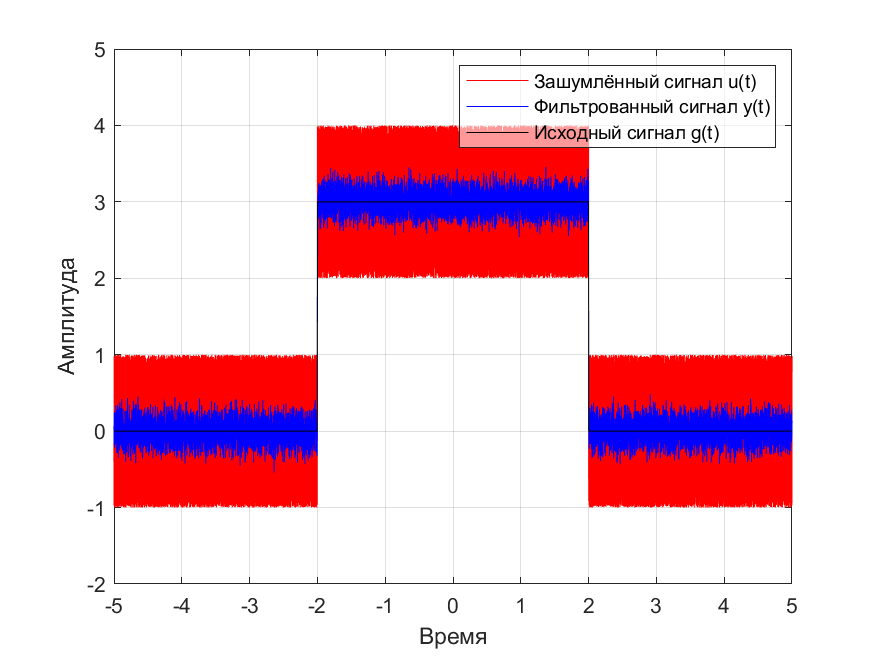
\includegraphics[width=\linewidth]{ex1_1/a=3_T=0.001/h1.png}
        \caption{$a = 3, T = 0.001$}
    \end{minipage}
    \begin{minipage}{0.5\textwidth}
        \centering
        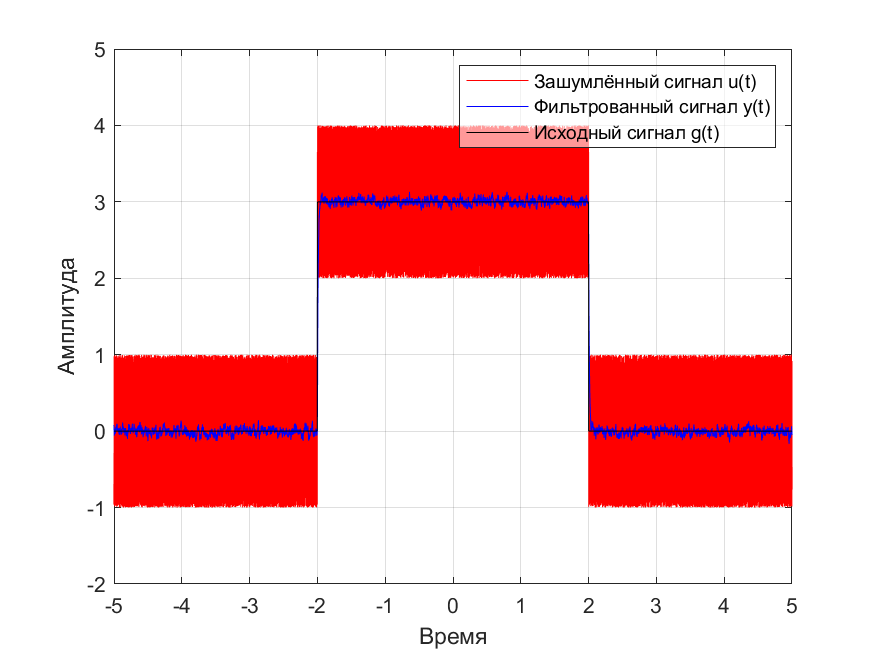
\includegraphics[width=\linewidth]{ex1_1/a=3_T=0.01/h1.png}
        \caption{$a = 3, T = 0.01$}
    \end{minipage}
\end{figure}

\begin{figure}[H]
    \begin{minipage}{0.5\textwidth}
        \centering
        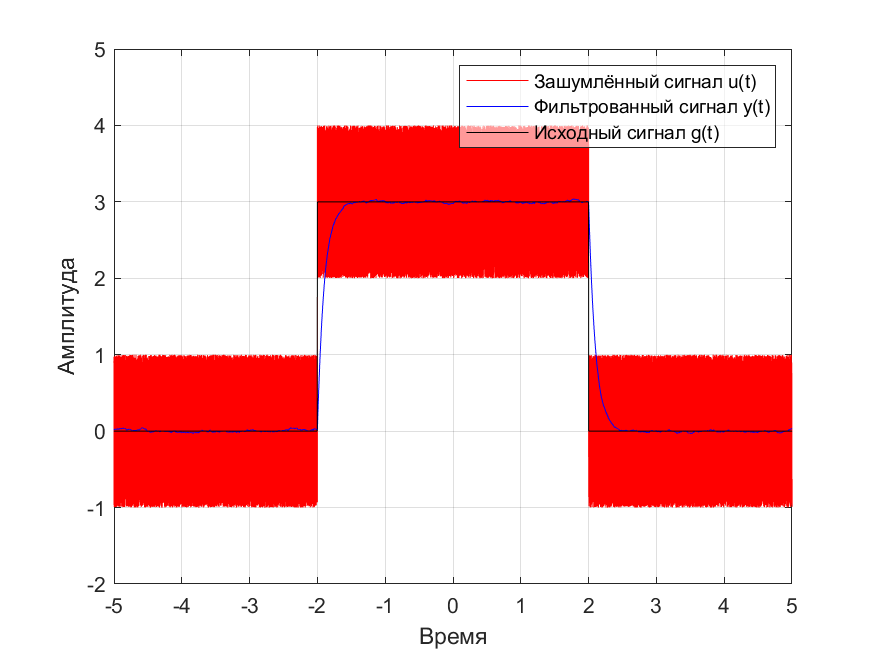
\includegraphics[width=\linewidth]{ex1_1/a=3_T=0.1/h1.png}
        \caption{$a = 3, T = 0.1$}
    \end{minipage}
    \begin{minipage}{0.5\textwidth}
        \centering
        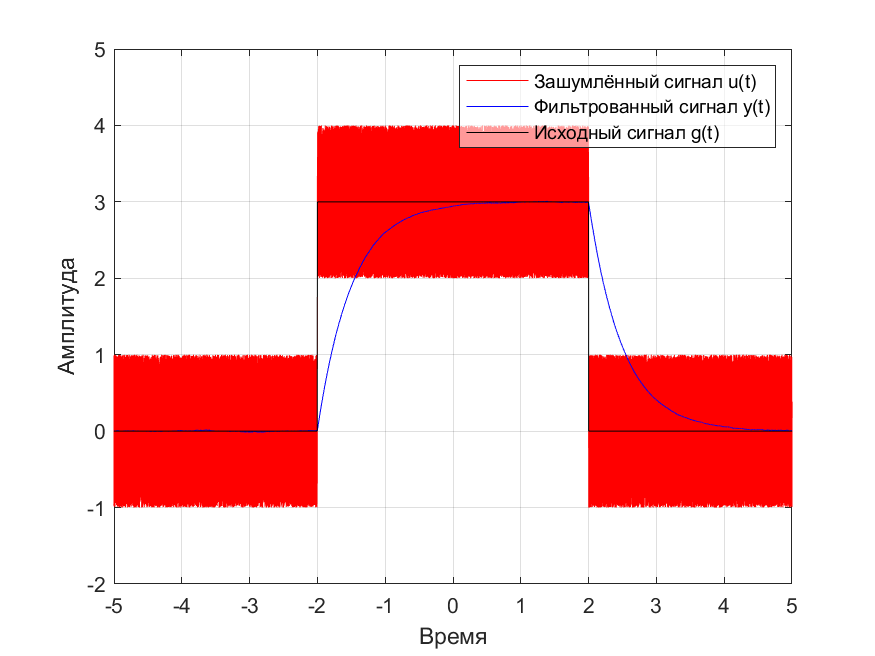
\includegraphics[width=\linewidth]{ex1_1/a=3_T=0.5/h1.png}
        \caption{$a = 3, T = 0.5$}
    \end{minipage}
\end{figure}

Видим, что при $T = 0.001$ фильтр оставляет слишком много шума, а при $T = 0.5$ функция теряет свой первоначальный облик, смещаясь с запозданием при скачках. Посмотрим на сравнительные графики модулей Фурье-образов этих сигналов: 

\begin{figure}[H]
    \begin{minipage}{0.5\textwidth}
        \centering
        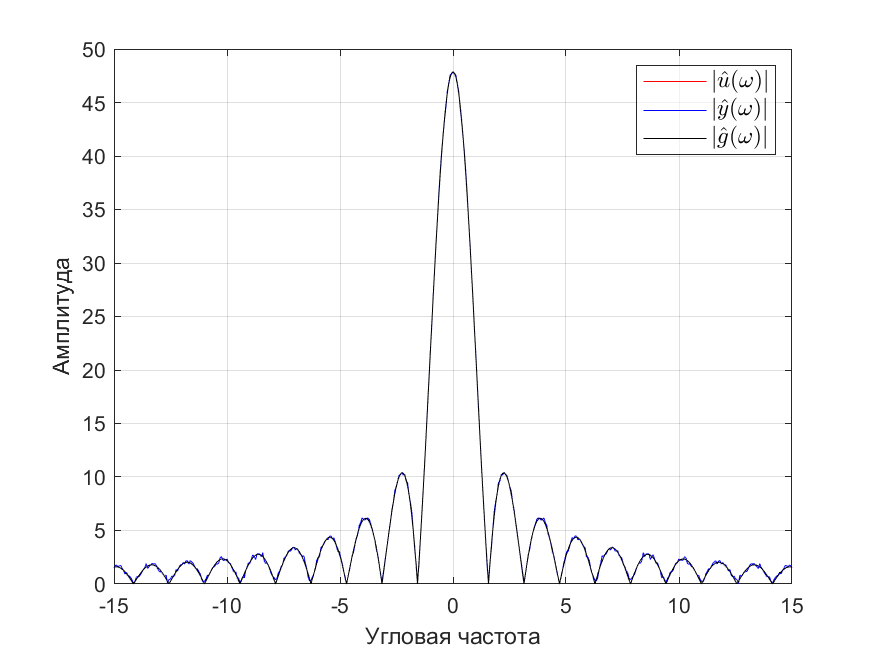
\includegraphics[width=\linewidth]{ex1_1/a=3_T=0.001/h3.png}
        \caption{$a = 3, T = 0.001$}
    \end{minipage}
    \begin{minipage}{0.5\textwidth}
        \centering
        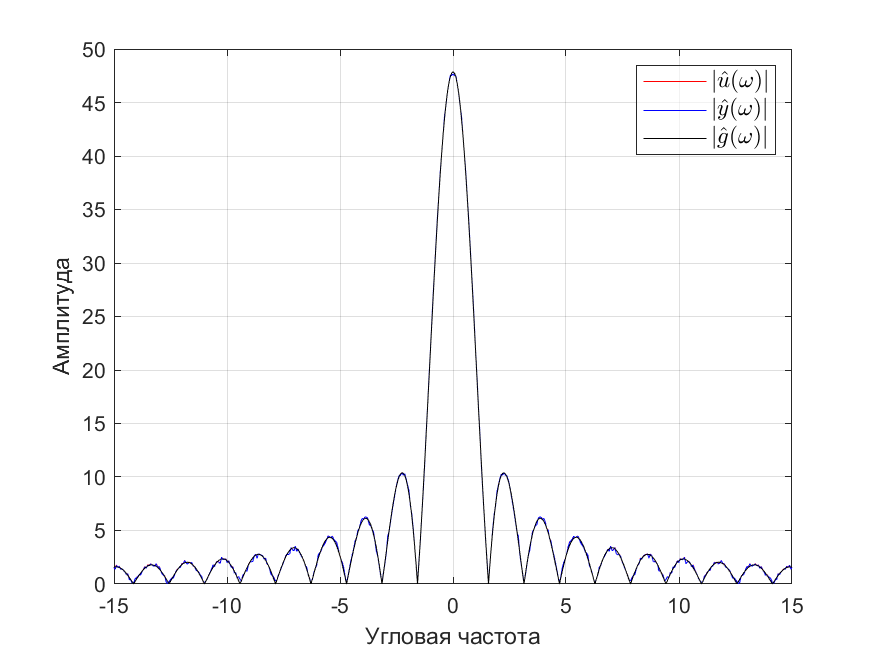
\includegraphics[width=\linewidth]{ex1_1/a=3_T=0.01/h3.png}
        \caption{$a = 3, T = 0.01$}
    \end{minipage}
\end{figure}

\begin{figure}[H]
    \begin{minipage}{0.5\textwidth}
        \centering
        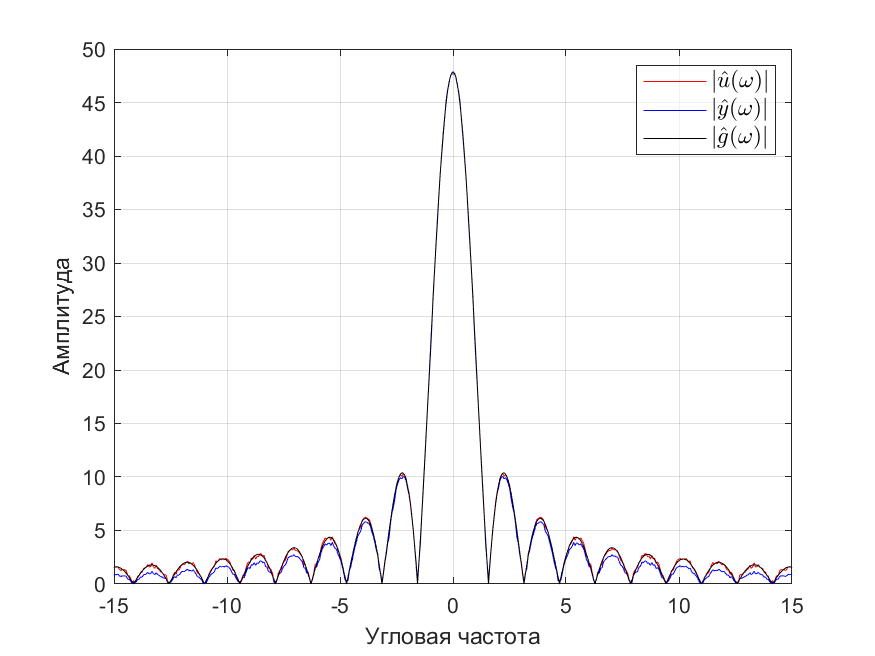
\includegraphics[width=\linewidth]{ex1_1/a=3_T=0.1/h3.png}
        \caption{$a = 3, T = 0.1$}
    \end{minipage}
    \begin{minipage}{0.5\textwidth}
        \centering
        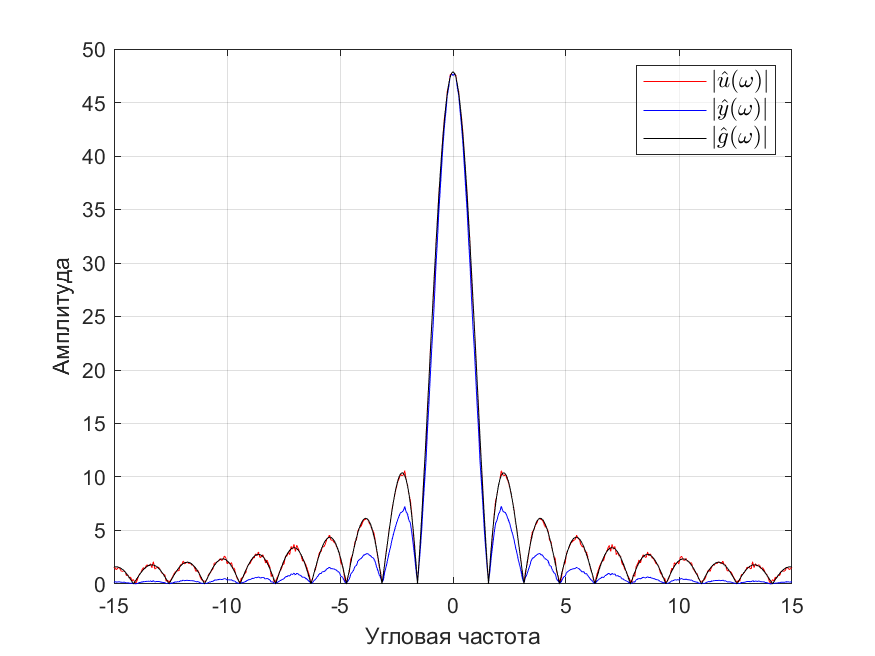
\includegraphics[width=\linewidth]{ex1_1/a=3_T=0.5/h3.png}
        \caption{$a = 3, T = 0.5$}
    \end{minipage}
\end{figure}

Заметно, что с увеличением $T$ уменьшается амплитуда фильтрованного сигнала, что показывает, почему отфильтрованная функция при $T = 0.5$ настолько отличается от оригинала -- низкие частоты сильно занижены.\ 

Посмотрим на сравнительные графики фильтрованного сигнала, полученного при помощи функции $lsim$ в $MATLAB$, и графики обратного преобразования Фурье от произведения $W_1(i\omega) \cdot \hat{u}(\omega)$:

\begin{figure}[H]
    \begin{minipage}{0.5\textwidth}
        \centering
        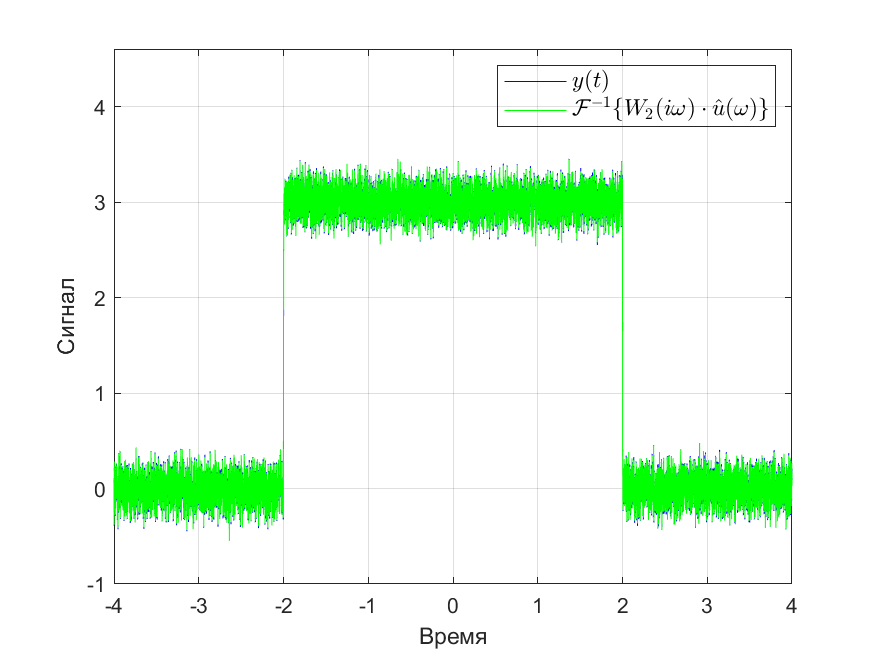
\includegraphics[width=\linewidth]{ex1_1/a=3_T=0.001/h2.png}
        \caption{$a = 3, T = 0.001$}
    \end{minipage}
    \begin{minipage}{0.5\textwidth}
        \centering
        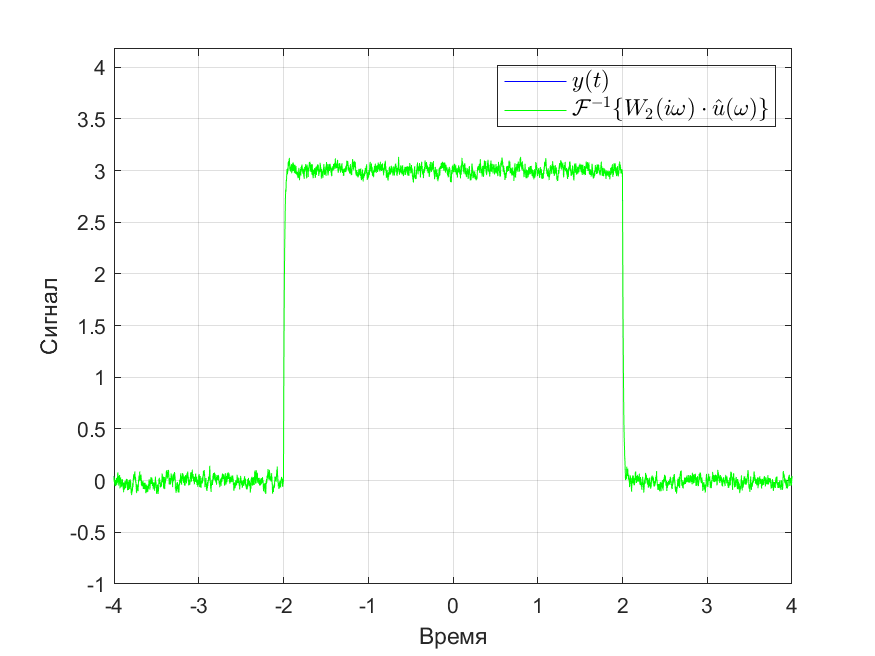
\includegraphics[width=\linewidth]{ex1_1/a=3_T=0.01/h2.png}
        \caption{$a = 3, T = 0.01$}
    \end{minipage}
\end{figure}

\begin{figure}[H]
    \begin{minipage}{0.5\textwidth}
        \centering
        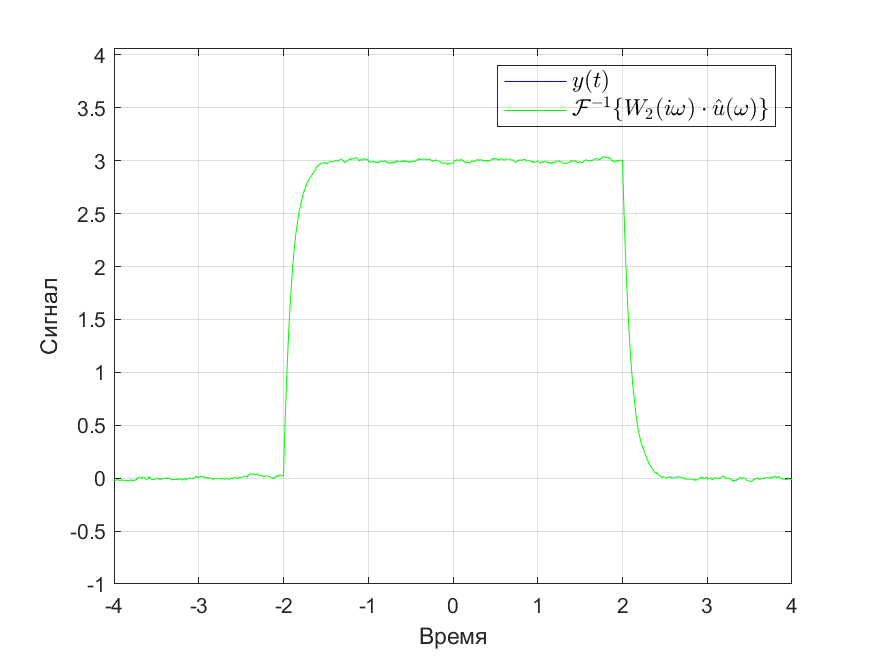
\includegraphics[width=\linewidth]{ex1_1/a=3_T=0.1/h2.png}
        \caption{$a = 3, T = 0.1$}
    \end{minipage}
    \begin{minipage}{0.5\textwidth}
        \centering
        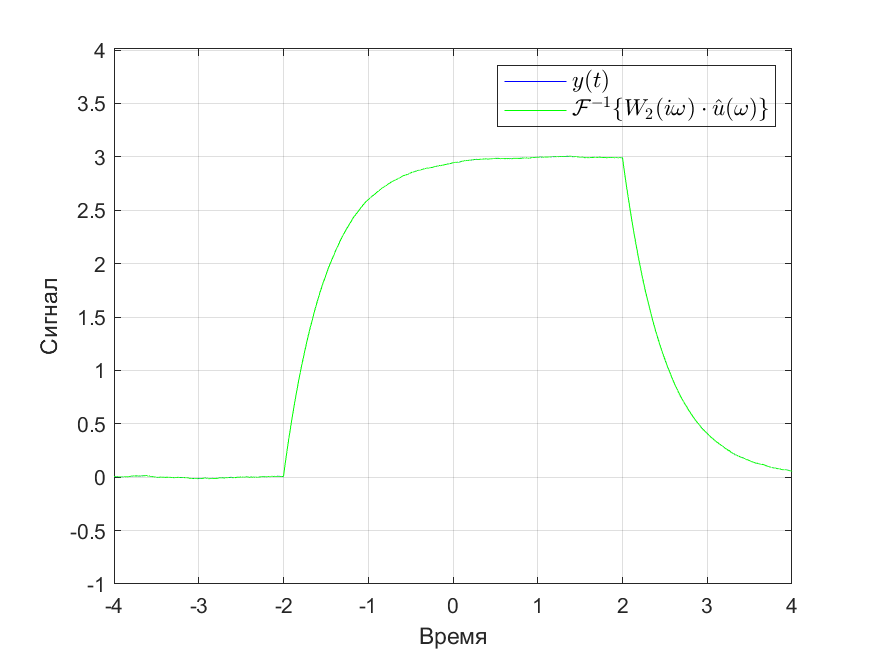
\includegraphics[width=\linewidth]{ex1_1/a=3_T=0.5/h2.png}
        \caption{$a = 3, T = 0.5$}
    \end{minipage}
\end{figure}

Видим, что обратное преобразование Фурье произведения частотной передаточной функции фильтра и образа зашумленного сигнала даёт в результате восстановленный сигнал. При $T = 0.001$ ещё можно заметить некоторые небольшие различия в получившихся функциях, в случае других $T$ приходится долго и мучительно увеличивать масштаб, чтобы увидеть хоть малейшее отличие между графиками, но эти отличия там точно есть, хоть функции и очень близки.\ 

Посмотрим на графики модулей Фурье-образов $y(t)$ и произведения $W_1(i\omega) \cdot \hat{u}(\omega)$:

\begin{figure}[H]
    \begin{minipage}{0.5\textwidth}
        \centering
        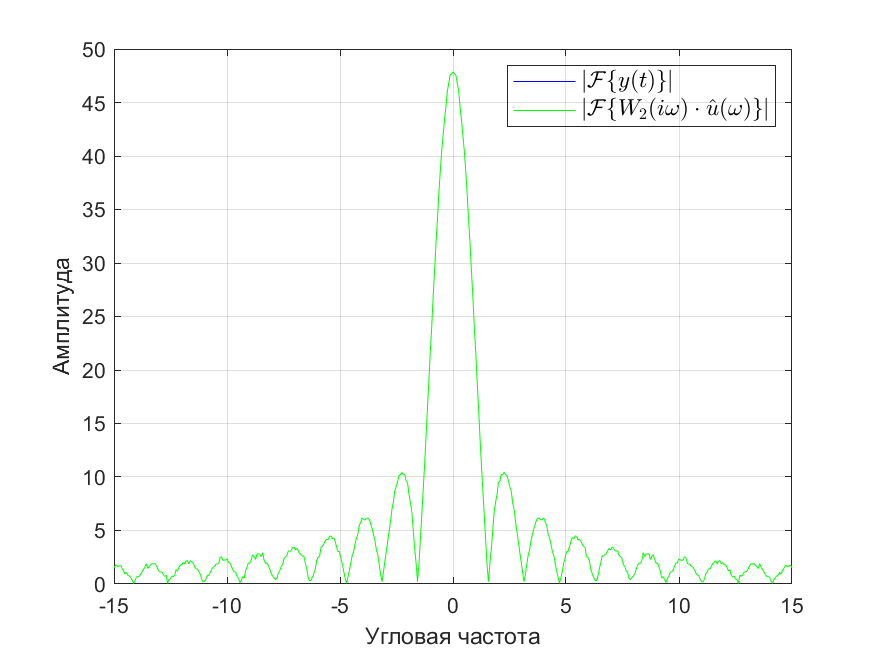
\includegraphics[width=\linewidth]{ex1_1/a=3_T=0.001/h4.png}
        \caption{$a = 3, T = 0.001$}
    \end{minipage}
    \begin{minipage}{0.5\textwidth}
        \centering
        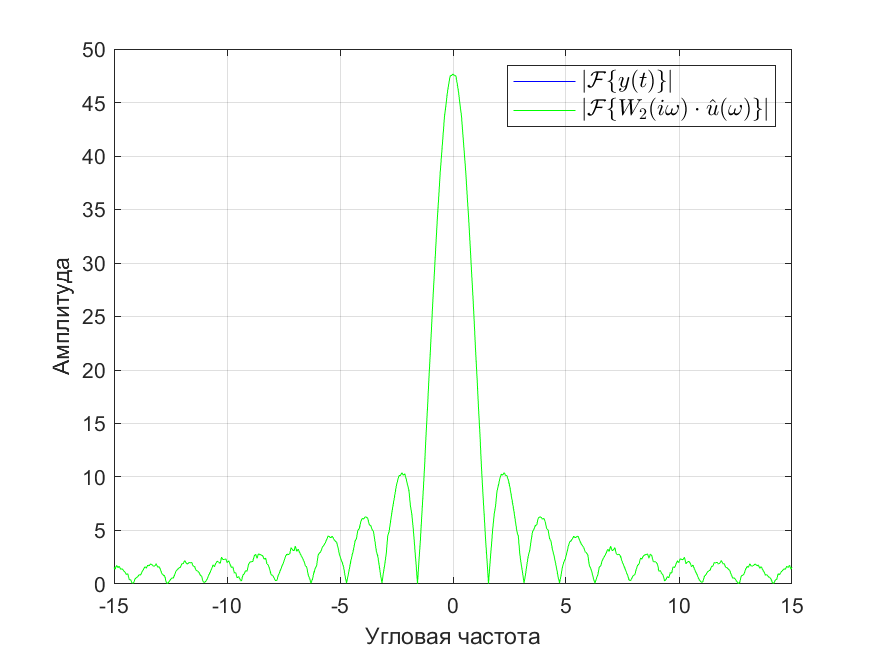
\includegraphics[width=\linewidth]{ex1_1/a=3_T=0.01/h4.png}
        \caption{$a = 3, T = 0.01$}
    \end{minipage}
\end{figure}

\begin{figure}[H]
    \begin{minipage}{0.5\textwidth}
        \centering
        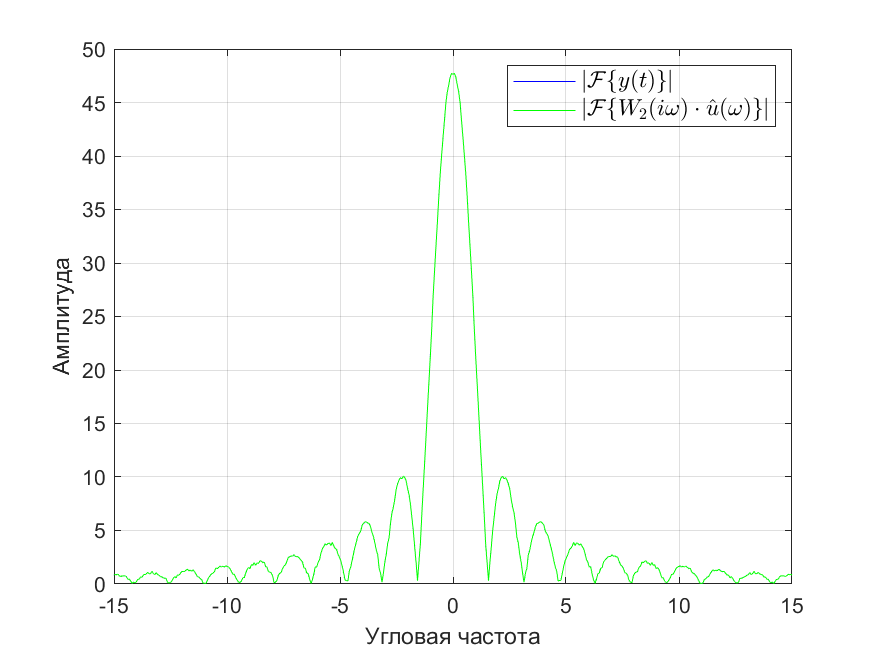
\includegraphics[width=\linewidth]{ex1_1/a=3_T=0.1/h4.png}
        \caption{$a = 3, T = 0.1$}
    \end{minipage}
    \begin{minipage}{0.5\textwidth}
        \centering
        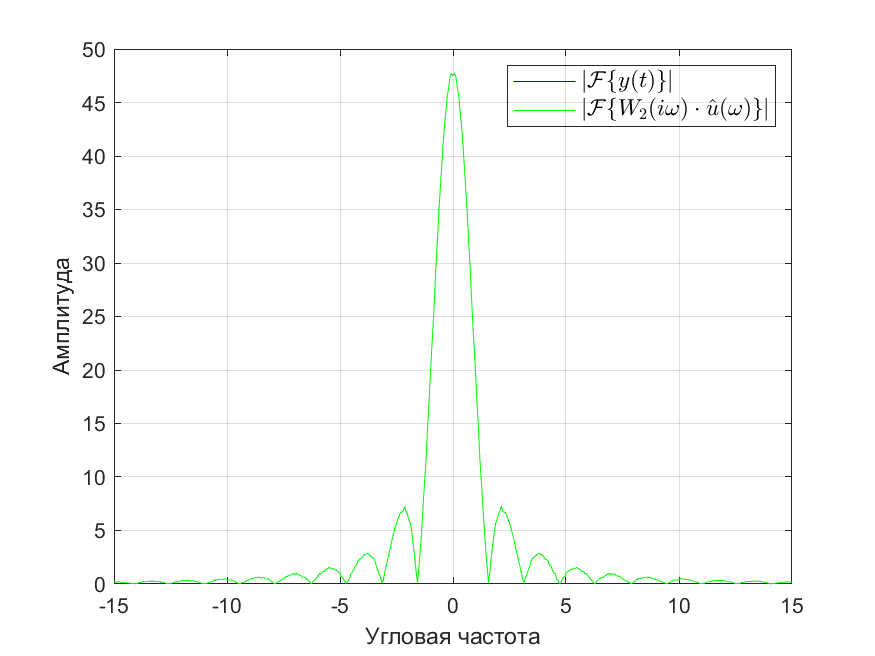
\includegraphics[width=\linewidth]{ex1_1/a=3_T=0.5/h4.png}
        \caption{$a = 3, T = 0.5$}
    \end{minipage}
\end{figure}

Набор данных $|\hat{y}(\omega)|$ уже был рассмотрен ранее, снова заметно уменьшение амплитуды при увеличении $T$. Разницы между $\left|\mathcal{F}\{y(t)\}\right|$ и $\left|\mathcal{F}\{W_1(i\omega) \cdot \hat{u}(\omega)\}\right|$ тут вовсе не видно. Максимальное расстояние между их графиками, которое мне удалось заметить -- около $0.001$\ 

Рассмотрим АЧХ фильтра для выбранных значений постоянной времени $T$:

\begin{figure}[H]
    \begin{minipage}{0.5\textwidth}
        \centering
        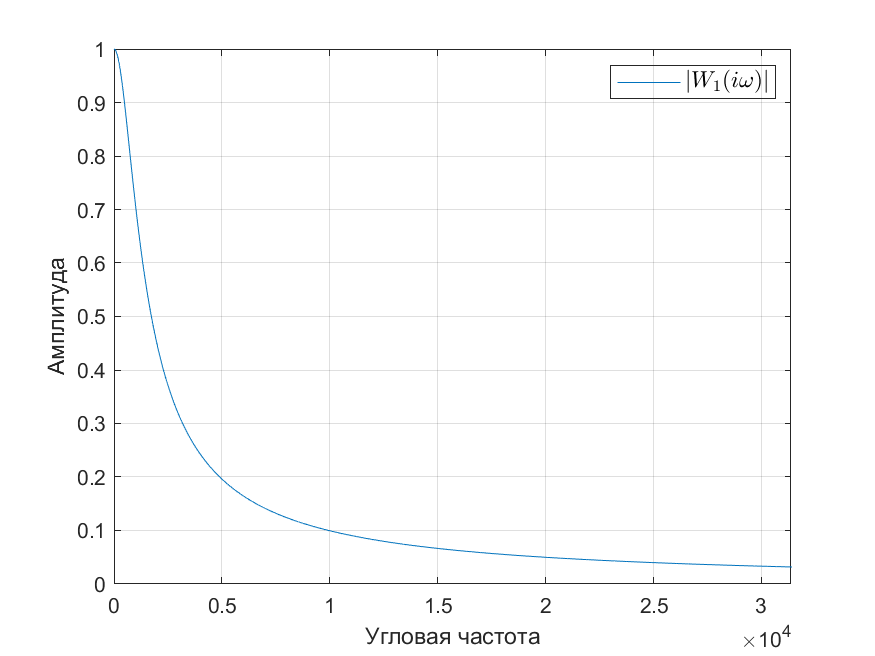
\includegraphics[width=\linewidth]{ex1_1/a=3_T=0.001/h5.png}
        \caption{$a = 3, T = 0.001$}
    \end{minipage}
    \begin{minipage}{0.5\textwidth}
        \centering
        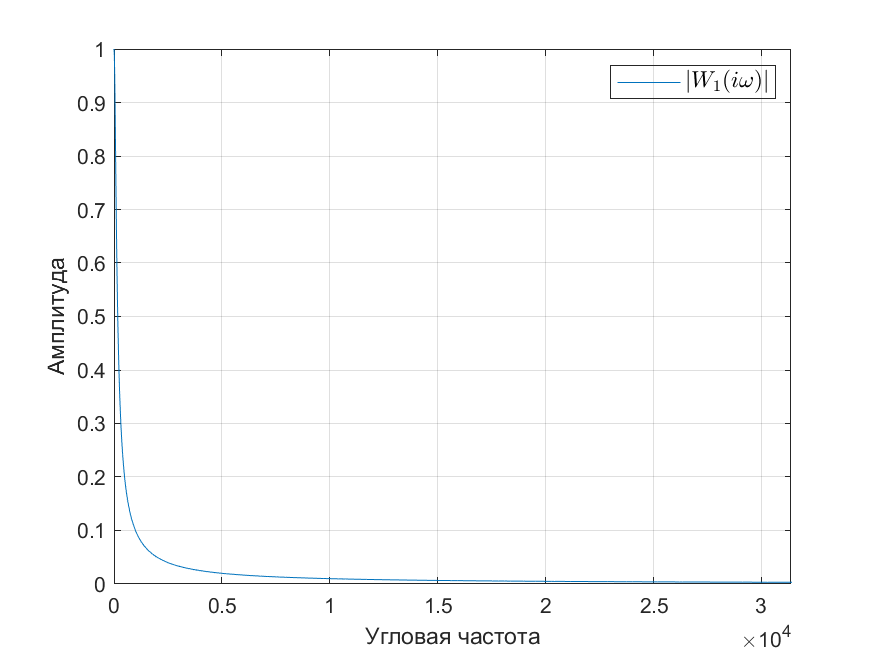
\includegraphics[width=\linewidth]{ex1_1/a=3_T=0.01/h5.png}
        \caption{$a = 3, T = 0.01$}
    \end{minipage}
\end{figure}

\begin{figure}[H]
    \begin{minipage}{0.5\textwidth}
        \centering
        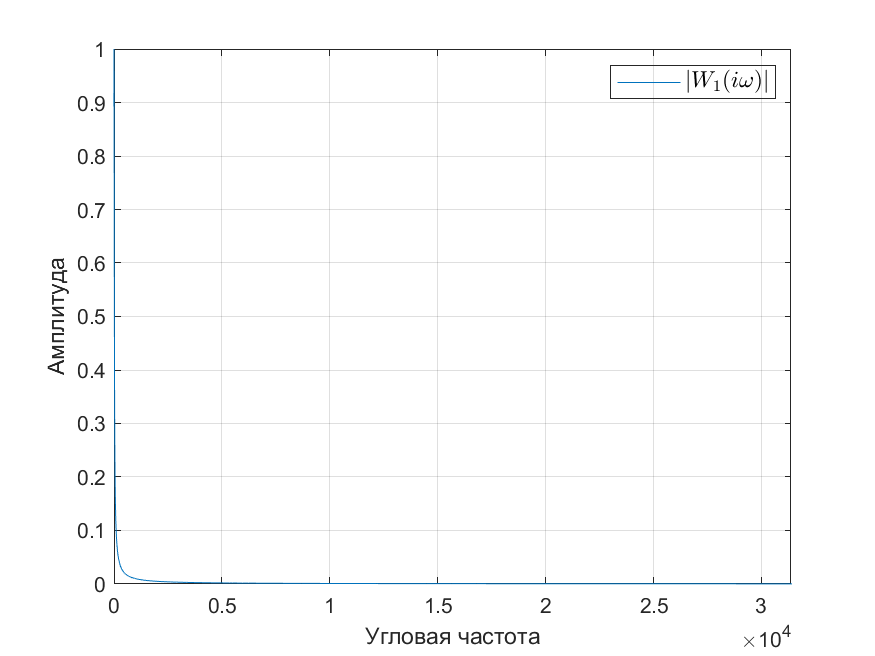
\includegraphics[width=\linewidth]{ex1_1/a=3_T=0.1/h5.png}
        \caption{$a = 3, T = 0.1$}
    \end{minipage}
    \begin{minipage}{0.5\textwidth}
        \centering
        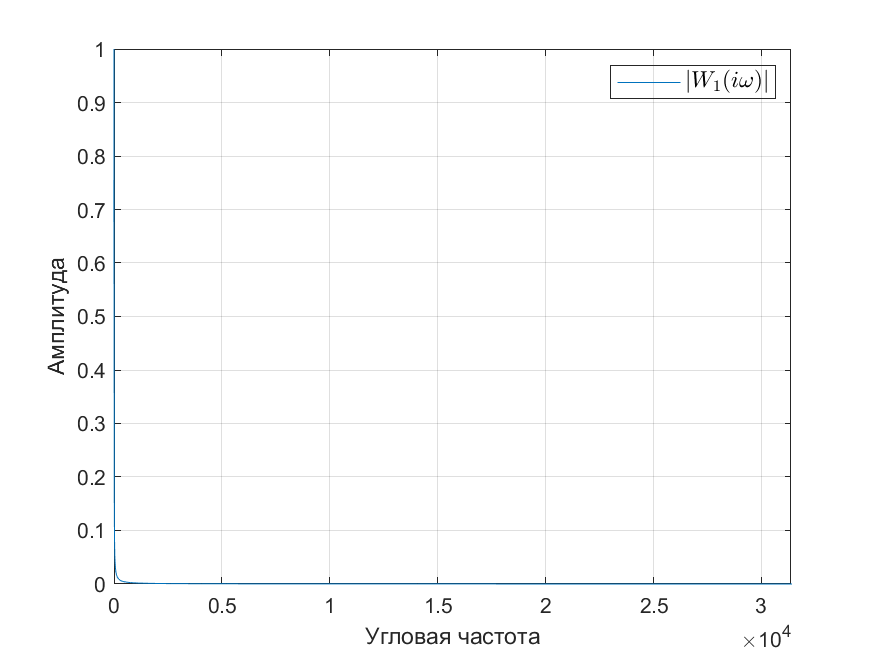
\includegraphics[width=\linewidth]{ex1_1/a=3_T=0.5/h5.png}
        \caption{$a = 3, T = 0.5$}
    \end{minipage}
\end{figure}

Видно, что с ростом $T$ количество частот, для которых сохраняется амплитуда, убывает. Притом меньшие частоты сохраняются в большей степени. Высокие частоты были срезаны почти всеми версиями фильтров. На основе этих графиков можно сказать, что при $T \to 0$ будет сохранено максимальное кол-во частот, то есть фильтр почти никак не повлияет на сигнал, а при увеличении $T$ будет урезаться всё больше частот, график АЧХ будет убывать всё быстрее.\

Лучшим же значением параметра $T$ для фильтра оказалось $0.01$ -- при таком значении фильтр не искажает исходную функцию как при $T = 0.1, 0.5$, довольно хорошо компенсируя шумы.
\subsubsection{Изучение влияния $a$}\

Примем $T = 0.01$, будем менять $a$, стараясь понять, как значение этого параметра влияет на эффективность фильтрации фильтром первого порядка. Брать значения для этого параметра будем из следующего списка: [-3, 0, 3, 20].
Для начала посмотрим на исходные графики и графики отфильтрованных сигналов: 

\begin{figure}[H]
    \begin{minipage}{0.5\textwidth}
        \centering
        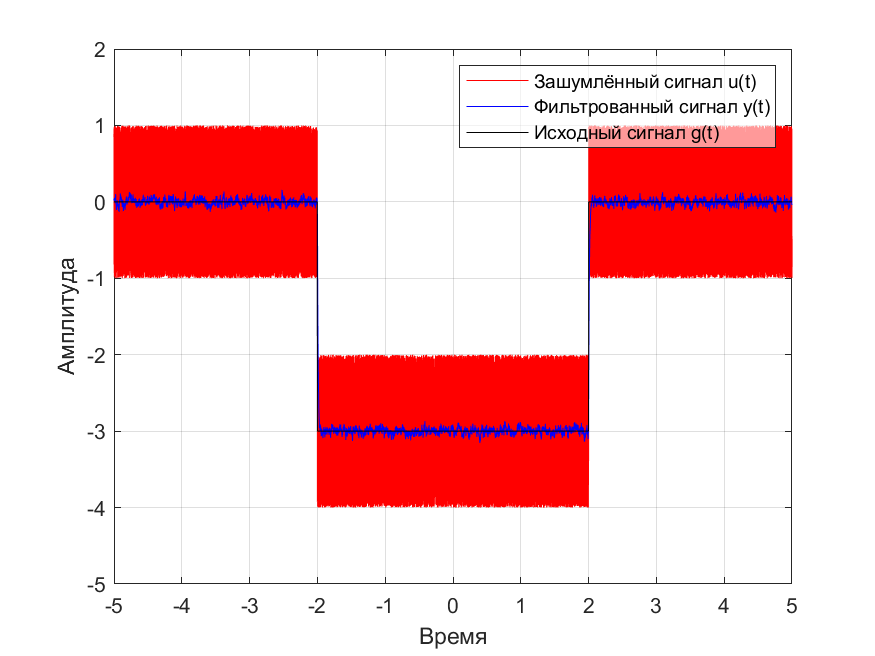
\includegraphics[width=\linewidth]{ex1_1/a=-3_T=0.01/h1.png}
        \caption{$a = -3, T = 0.01$}
    \end{minipage}
    \begin{minipage}{0.5\textwidth}
        \centering
        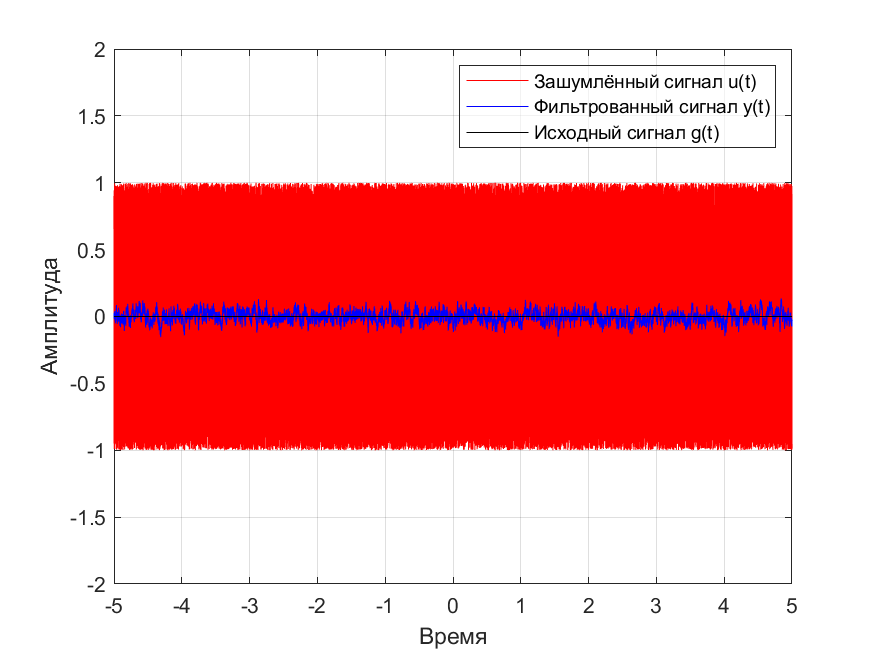
\includegraphics[width=\linewidth]{ex1_1/a=0_T=0.01/h1.png}
        \caption{$a = 0, T = 0.01$}
    \end{minipage}
\end{figure}

\begin{figure}[H]
    \begin{minipage}{0.5\textwidth}
        \centering
        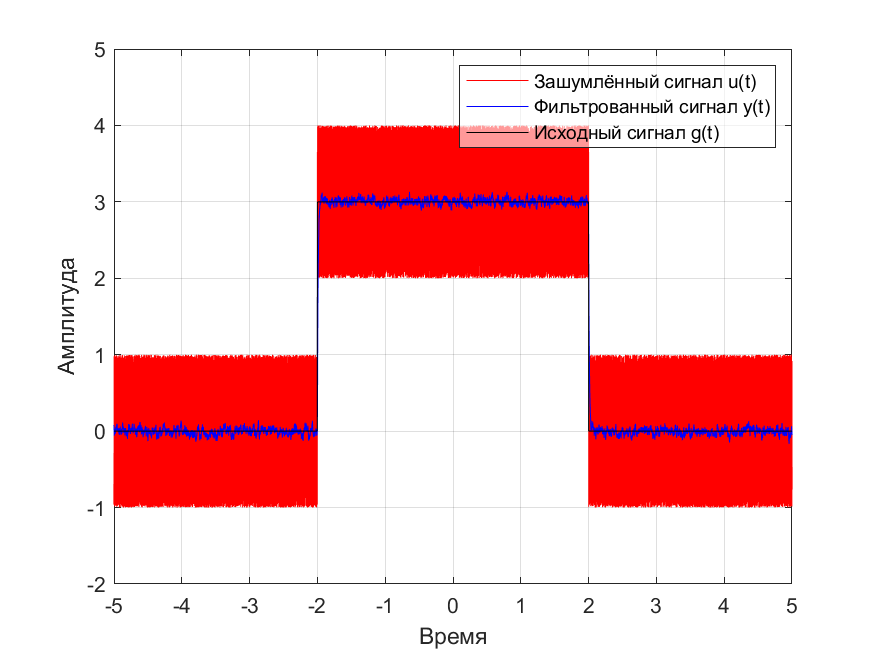
\includegraphics[width=\linewidth]{ex1_1/a=3_T=0.01/h1.png}
        \caption{$a = 3, T = 0.01$}
    \end{minipage}
    \begin{minipage}{0.5\textwidth}
        \centering
        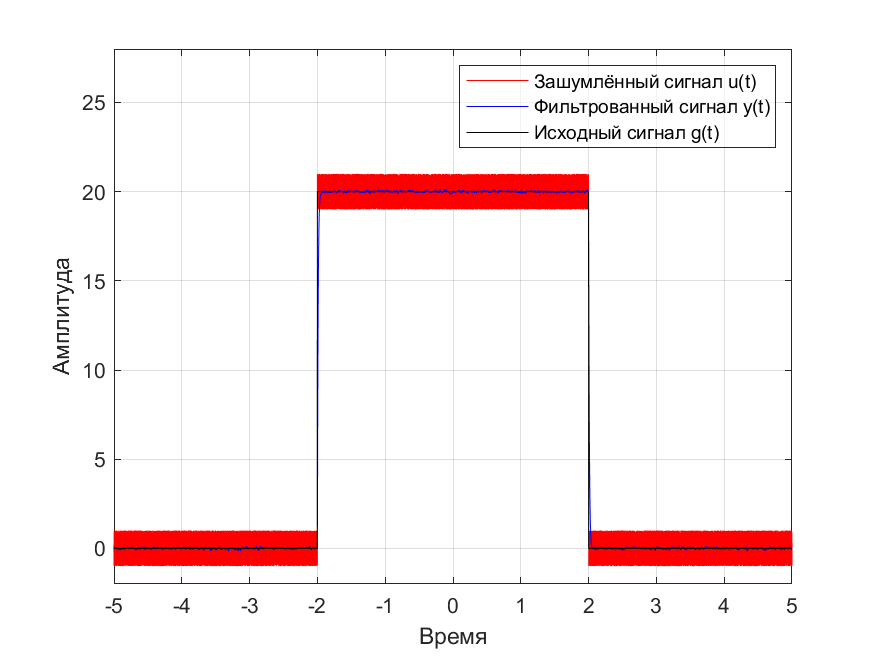
\includegraphics[width=\linewidth]{ex1_1/a=20_T=0.01/h1.png}
        \caption{$a = 20, T = 0.01$}
    \end{minipage}
\end{figure}

Пока что особых изменений не заметно, посмотрим на графики модулей Фурье-образов этих функций:

\begin{figure}[H]
    \begin{minipage}{0.5\textwidth}
        \centering
        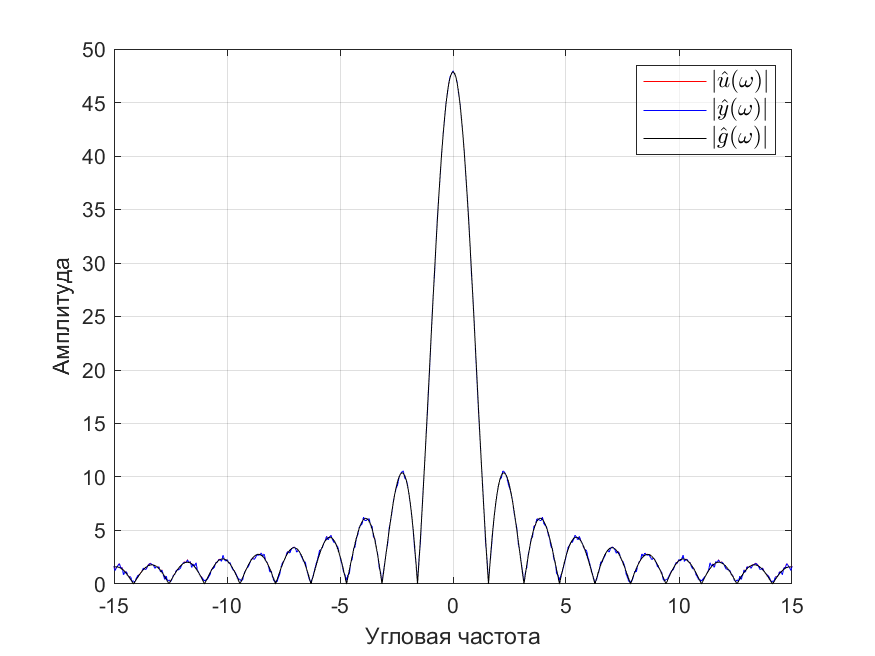
\includegraphics[width=\linewidth]{ex1_1/a=-3_T=0.01/h3.png}
        \caption{$a = -3, T = 0.01$}
    \end{minipage}
    \begin{minipage}{0.5\textwidth}
        \centering
        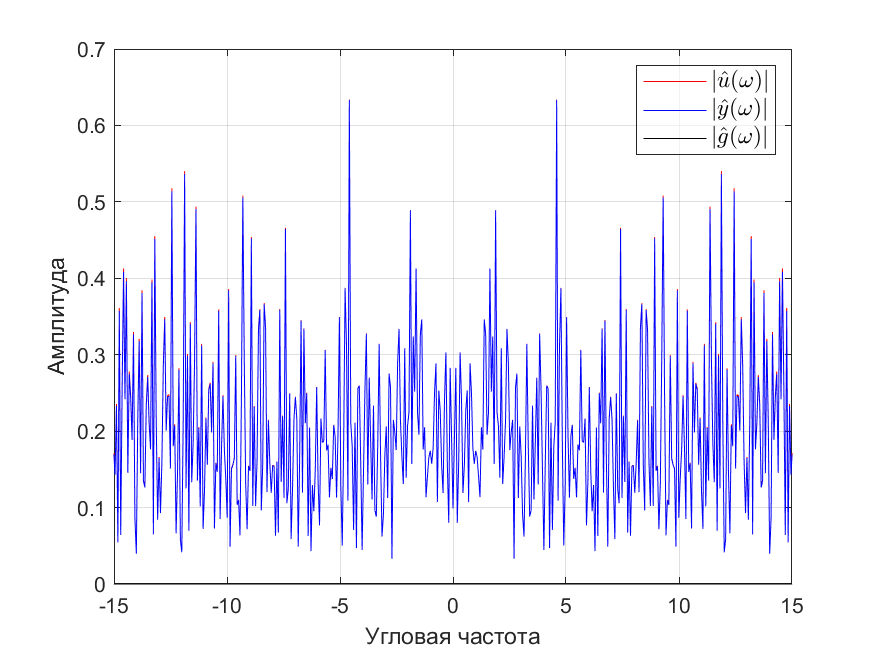
\includegraphics[width=\linewidth]{ex1_1/a=0_T=0.01/h3.png}
        \caption{$a = 0, T = 0.01$}
    \end{minipage}
\end{figure}

\begin{figure}[H]
    \begin{minipage}{0.5\textwidth}
        \centering
        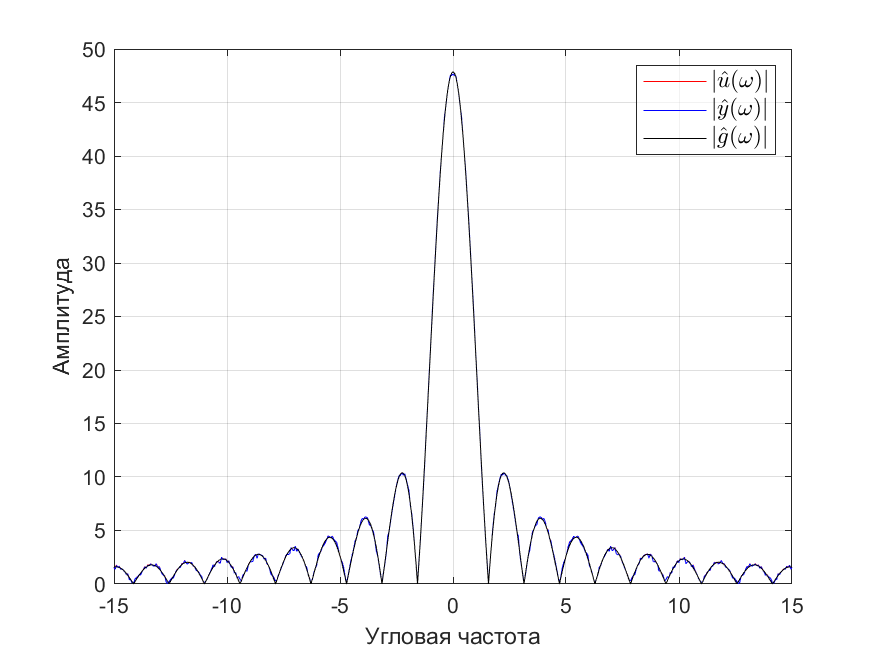
\includegraphics[width=\linewidth]{ex1_1/a=3_T=0.01/h3.png}
        \caption{$a = 3, T = 0.01$}
    \end{minipage}
    \begin{minipage}{0.5\textwidth}
        \centering
        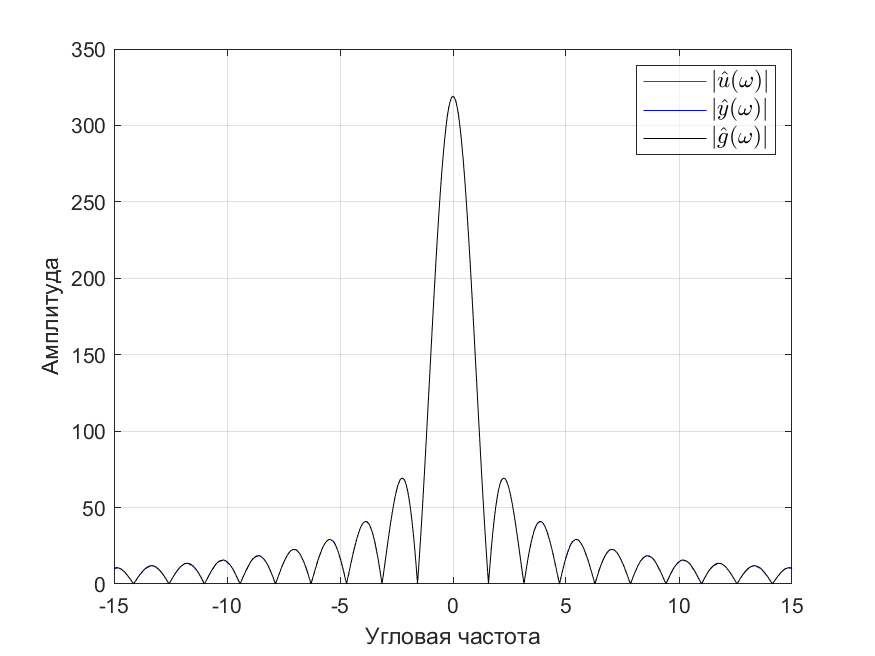
\includegraphics[width=\linewidth]{ex1_1/a=20_T=0.01/h3.png}
        \caption{$a = 20, T = 0.01$}
    \end{minipage}
\end{figure}

Заметно, что чем больше значение параметра $a$, тем больше амплитуда модуля Фурье-образа функции $u(t)$ и её отфильтрованного варианта, также графики модулей образов при $a = -3$ и при $a = 3$ идентичны, при $a = 0$ модуль Фурье-образа исходной $g(t)$ равен нулю.

Посмотрим на графики фильтрованного сигнала, полученного при помощи функции $lsim$ в $MATLAB$, и графики обратного преобразования Фурье от произведения $W_1(i\omega) \cdot \hat{u}(\omega)$:

\begin{figure}[H]
    \begin{minipage}{0.5\textwidth}
        \centering
        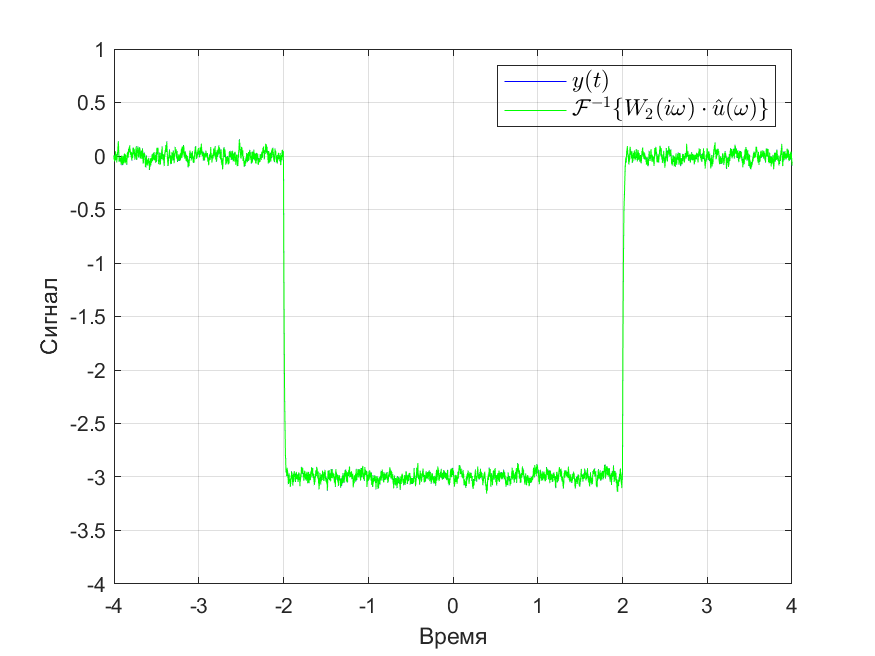
\includegraphics[width=\linewidth]{ex1_1/a=-3_T=0.01/h2.png}
        \caption{$a = -3, T = 0.01$}
    \end{minipage}
    \begin{minipage}{0.5\textwidth}
        \centering
        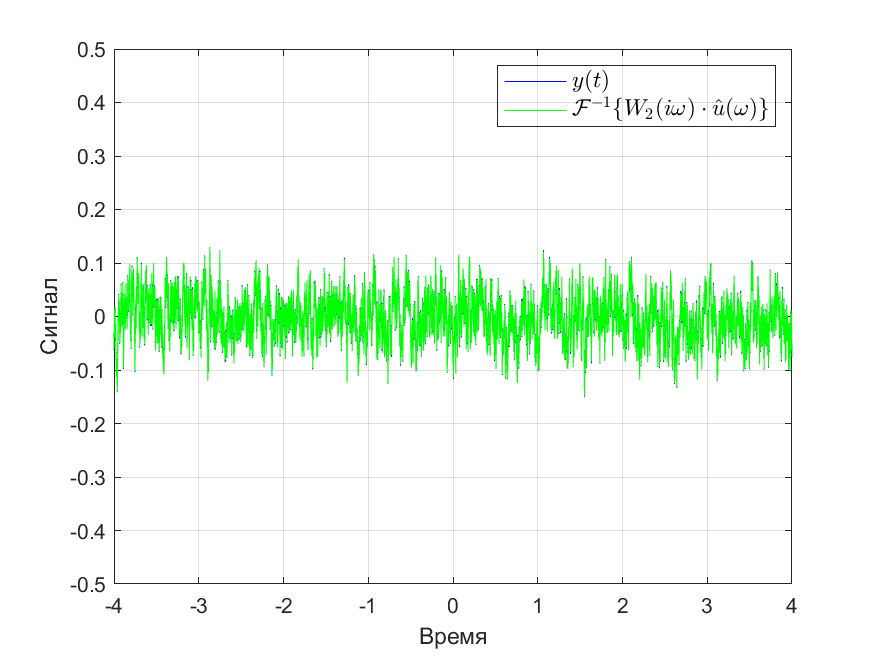
\includegraphics[width=\linewidth]{ex1_1/a=0_T=0.01/h2.png}
        \caption{$a = 0, T = 0.01$}
    \end{minipage}
\end{figure}

\begin{figure}[H]
    \begin{minipage}{0.5\textwidth}
        \centering
        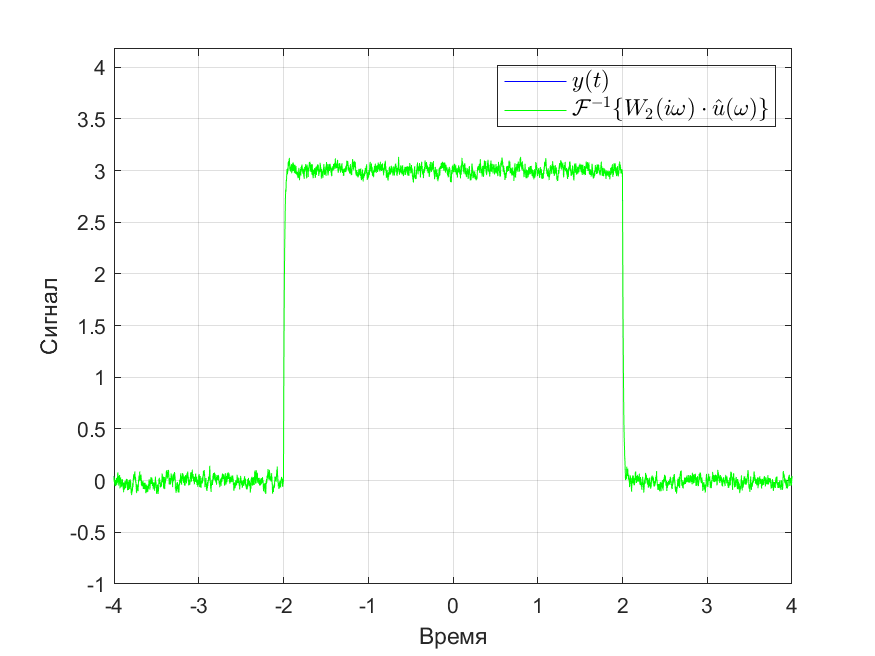
\includegraphics[width=\linewidth]{ex1_1/a=3_T=0.01/h2.png}
        \caption{$a = 3, T = 0.01$}
    \end{minipage}
    \begin{minipage}{0.5\textwidth}
        \centering
        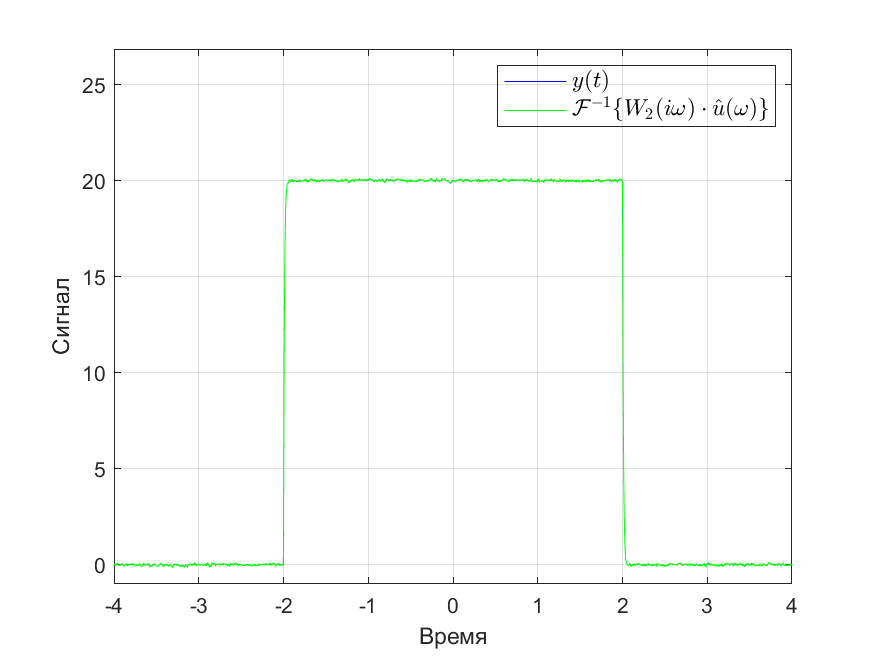
\includegraphics[width=\linewidth]{ex1_1/a=20_T=0.01/h2.png}
        \caption{$a = 20, T = 0.01$}
    \end{minipage}
\end{figure}

При выбранном масштабе кажется, что при $a = 20$ фильтр избавляет функцию от шумов гораздо лучше, чем при меньших значениях, однако, если увеличить масштаб графика, станет понятно, что помехи меньше не стали. Теперь настала очередь модулей Фурье-образов функций, соответствующих только что рассмотренным:

\begin{figure}[H]
    \begin{minipage}{0.5\textwidth}
        \centering
        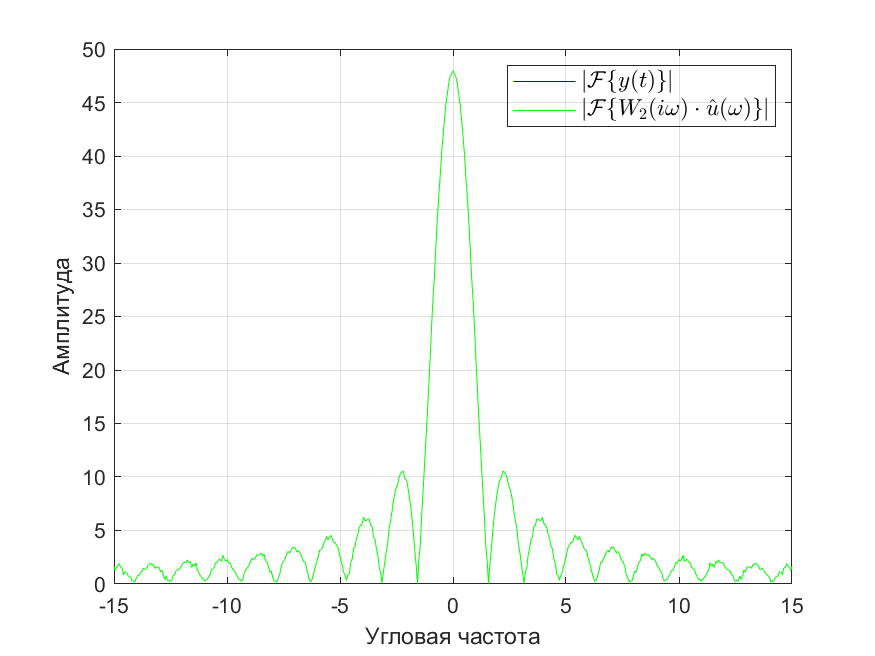
\includegraphics[width=\linewidth]{ex1_1/a=-3_T=0.01/h4.png}
        \caption{$a = -3, T = 0.01$}
    \end{minipage}
    \begin{minipage}{0.5\textwidth}
        \centering
        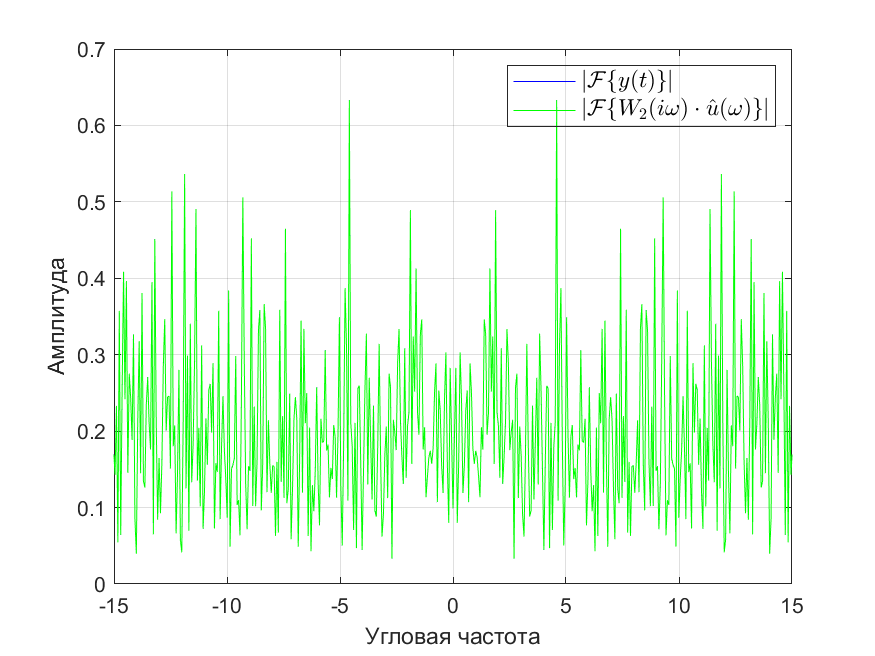
\includegraphics[width=\linewidth]{ex1_1/a=0_T=0.01/h4.png}
        \caption{$a = 0, T = 0.01$}
    \end{minipage}
\end{figure}

\begin{figure}[H]
    \begin{minipage}{0.5\textwidth}
        \centering
        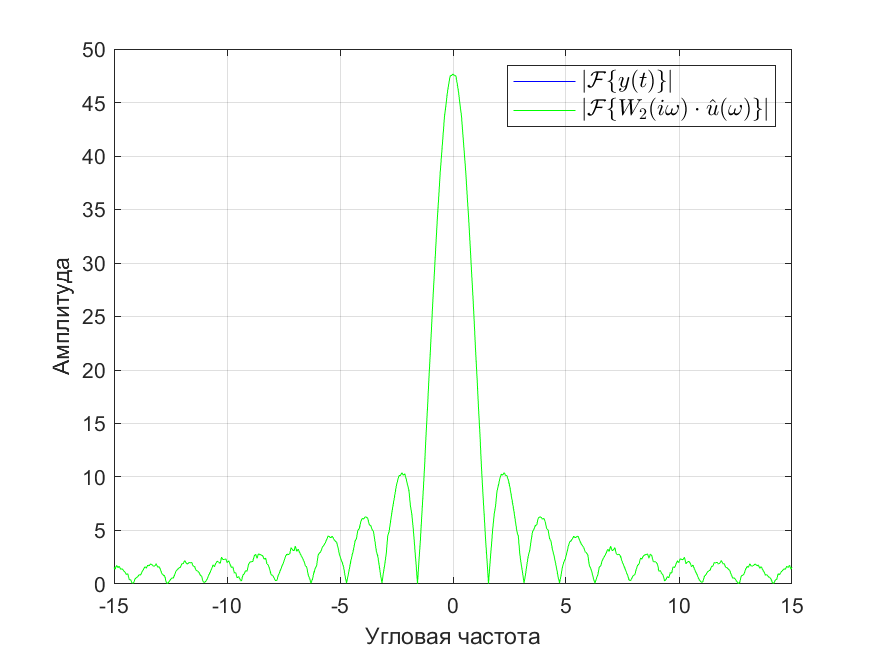
\includegraphics[width=\linewidth]{ex1_1/a=3_T=0.01/h4.png}
        \caption{$a = 3, T = 0.01$}
    \end{minipage}
    \begin{minipage}{0.5\textwidth}
        \centering
        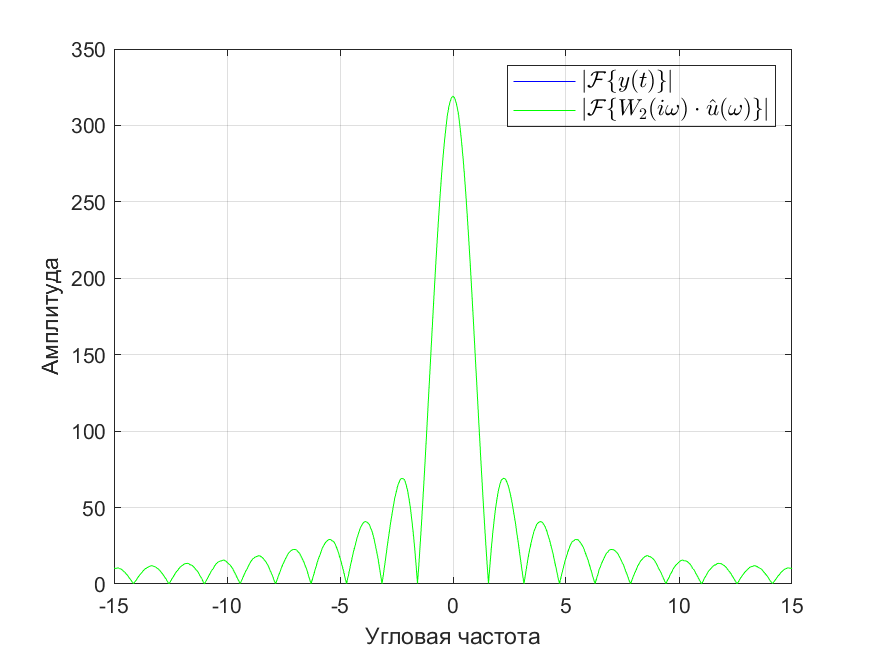
\includegraphics[width=\linewidth]{ex1_1/a=20_T=0.01/h4.png}
        \caption{$a = 20, T = 0.01$}
    \end{minipage}
\end{figure}

Видим, что различия между графиками снова незначительные, в рамках погрешности. Влияние коэффициента $a$ также понятно -- чем он больше, тем больше амплитуда модулей рассмотренных Фурье-образов. График АЧХ фильтра же останется неизменным для всех $a$ -- он не зависит от рассматриваемых сигналов, подаваемых на вход фильтру, а значит, не зависит и от коэффициента $a$.

\subsubsection{Вывод}\

Постоянная времени $T$ отвечает за динамику фильтра: чем больше $T$, тем более плавным будет отклик фильтра, что позволяет снизить шум, но может ослабить отклик на быстрые изменения в сигнале. Параметр $a$ в функции $g(t)$ определяет амплитуду сигнала. Увеличение значения $a$ увеличивает амплитуду сигнала, что делает его более выраженным на фоне шума, но на эффективность фильтрации напрямую не влияет.

\subsection{Режекторный полосовой фильтр}\

В этом пункте, в отличие от предыдущего, шумы к функции добавляются лишь гармонические ($b = 0$), соответственно, функция $u(t)$ принимает следующий вид:

$$
u(t) = g(t) + c\sin{(dt)}
$$\ 

Также в задании вместо линейного фильтра первого порядка используется фильтр второго порядка, вот как выглядит соответствующая ему передаточная функция:

$$
W_2(p) = \frac{p^2 + a_1p + a_2}{p^2 + b_1p + b_2},
$$
при этом $a_1, a_2, b_1, b_2$ должны быть выбраны так, что:

\begin{enumerate}
    \item Корни полинома знаменателя $p_1, p_2$ должны иметь строго отрицательную вещественную часть.
    \item Для нижних частот $(\omega \to 0)$ и верхних частот $(\omega \to \infty)$ АЧХ фильтра должна быть равна $1$.
    \item Для некоторой частоты $\omega_0$ АЧХ фильтра должна быть равна $0$.
\end{enumerate}\

Корни полинома знаменателя имеют отрицательную вещественную часть тогда и только тогда, когда $b_1, b_2 > 0$. А существование этих корней будет гарантировать положительный дискриминант

$$D = b_1^2-4b_2 > 0 \Leftrightarrow |b_1| > 2 \sqrt{b_2}.$$\ 

Для проверки второго и третьего условий проанализируем АЧХ фильтра, для чего перейдём к частотной передаточной функции, а затем найдем её вещественную и мнимую части путём домножения на сопряжённое к знаменателю, получим

$$
W(i\omega) = \frac{\omega^{4\ }+\ \omega^{2}\left(-b_{2}+a_{1}b_{1}-a_{2}\right)+a_{2}b_{2} + i\omega^{3}\left(b_{1}-a_{1}\right)+i\omega\left(a_{1}b_{2}-a_{2}b_{1}\right)}{\omega^{4}+\omega^{2}\left(b_{1}^{2}-2b_{2}\right)+b_{2}^{2}};$$
$$
W(i\omega) = P(\omega) + i Q(\omega),
$$

откуда
$$
P(\omega) = \frac{\omega^{4\ }+\ \omega^{2}\left(-b_{2}+a_{1}b_{1}-a_{2}\right)+a_{2}b_{2}}{\omega^{4}+\omega^{2}\left(b_{1}^{2}-2b_{2}\right)+b_{2}^{2}}, \
Q(\omega) = \frac{\omega^{3}\left(b_{1}-a_{1}\right)+\omega\left(a_{1}b_{2}-a_{2}b_{1}\right)}{x^{4}+x^{2}\left(b_{1}^{2}-2b_{2}\right)+b_{2}^{2}}.
$$

Рассмотрим пределы:

$$
\lim_{\limits{\omega \to 0}} P(\omega) = \frac{a_2b_2}{b_2^2} = \frac{a_2}{b_2}, \,
\lim_{\limits{\omega \to 0}} Q(\omega) = 0.
$$

Амплитуда передаточной функции:

$$
\left| W(i \omega)\right| = \sqrt{P^2(\omega) + Q^2(\omega)}.
$$

Тогда выполнение условия

$$\lim_{\limits{\omega \to 0}} \left| W(i \omega)\right| = 1$$

равносильно выполнению

$$\lim_{\limits{\omega \to 0}} \sqrt{P^2(\omega) + Q^2(\omega)} = \sqrt{\left(\frac{a_2}{b_2}\right)^2 + 0^2} = \left| \frac{a_2}{b_2}\right| = 1 \Rightarrow a_2 = \pm b_2.$$

Рассмотрим пределы при $\omega \to \infty$:

$$
\lim_{\limits{\omega \to \infty}} P(\omega) = 1, \,
\lim_{\limits{\omega \to \infty}} Q(\omega) = 0
$$

Они не зависят от рассматриваемых переменных параметров, при этом всегда выполняется

$$
\lim_{\limits{\omega \to \infty}} \left| W(i \omega)\right| = 1.
$$

Следовательно, это условие не повлияет на выбор значений параметров.

Третье же условие выполняется, когда $a_1 = 0$ и $a_2 = b_2$. При этом частота $\omega_0$ будет равна $\sqrt{a_2}$ (при таком значении $\omega$ числитель АЧХ равен нулю).

Итак, итоговые условия для выбора значений параметров: $a_1 = 0, b_1 > 0, \, b_2 > 0, \, b_1 > 2\sqrt{b_2}, a_2 = b_2$.

Для начала возьмём значения параметров $a_1, a_2, b_2$ равными $0, 2500, 2500$ соответственно. Рассмотрим влияние значения $b_1$ на график АЧХ:

\begin{figure}[H]
    \begin{minipage}{0.5\textwidth}
        \centering
        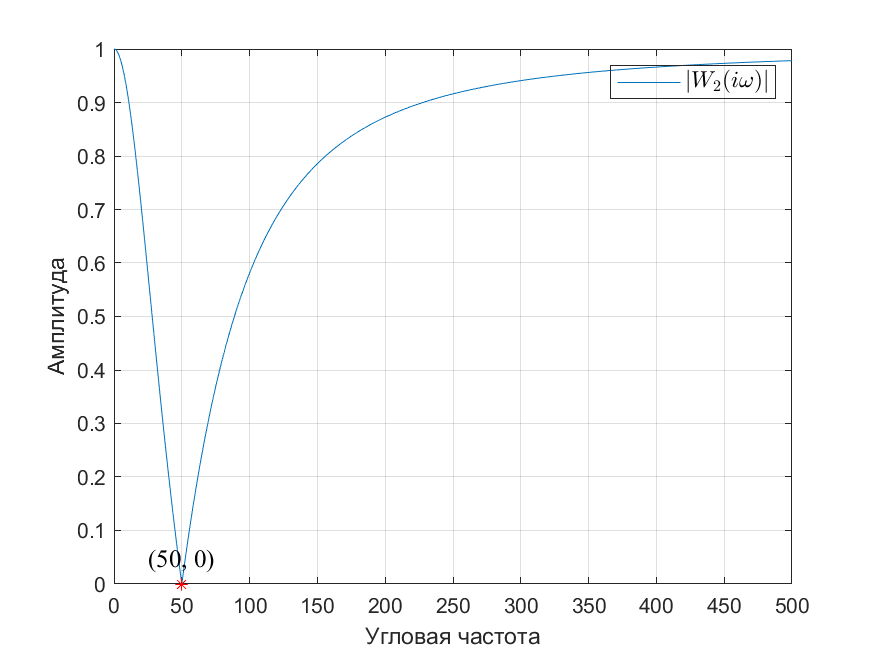
\includegraphics[width=\linewidth]{ex1_2/a1=0_a2=2500_b1=105_b2=2500_d=50/h1.png}
        \caption{$a_1=0, a_2=2500, b_1=105, b_2=2500$}
    \end{minipage}
    \begin{minipage}{0.5\textwidth}
        \centering
        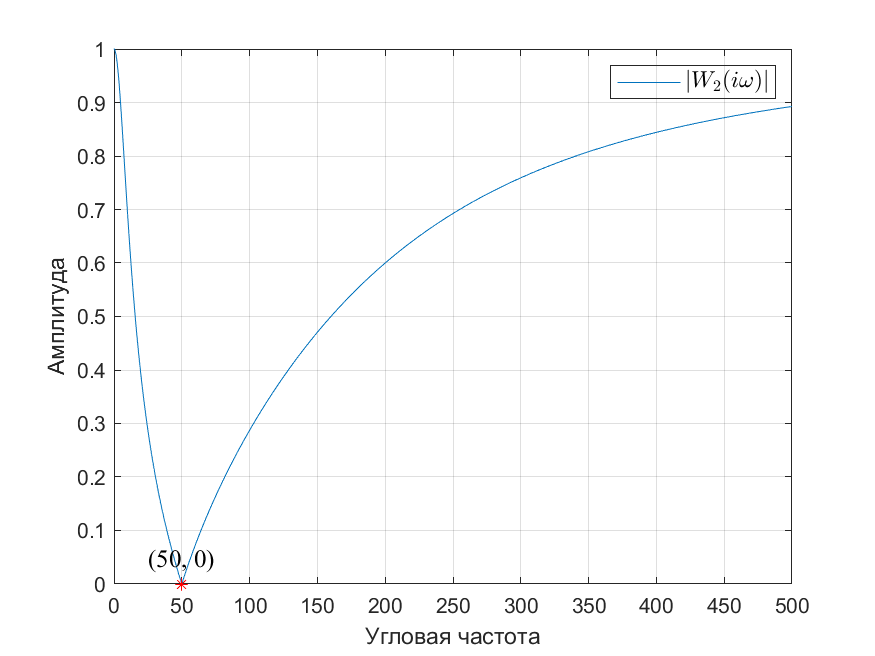
\includegraphics[width=\linewidth]{ex1_2/a1=0_a2=2500_b1=250_b2=2500_d=50/h1.png}
        \caption{$a_1=0, a_2=2500, b_1=250, b_2=2500$}
    \end{minipage}
\end{figure}

\begin{figure}[H]
    \begin{minipage}{0.5\textwidth}
        \centering
        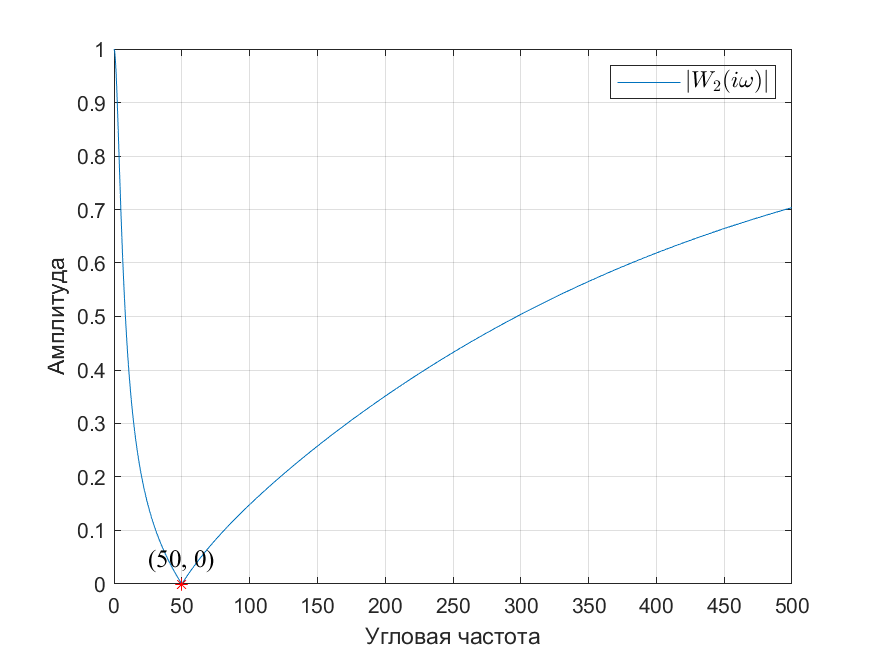
\includegraphics[width=\linewidth]{ex1_2/a1=0_a2=2500_b1=500_b2=2500_d=50/h1.png}
        \caption{$a_1=0, a_2=2500, b_1=500, b_2=2500$}
    \end{minipage}
    \begin{minipage}{0.5\textwidth}
        \centering
        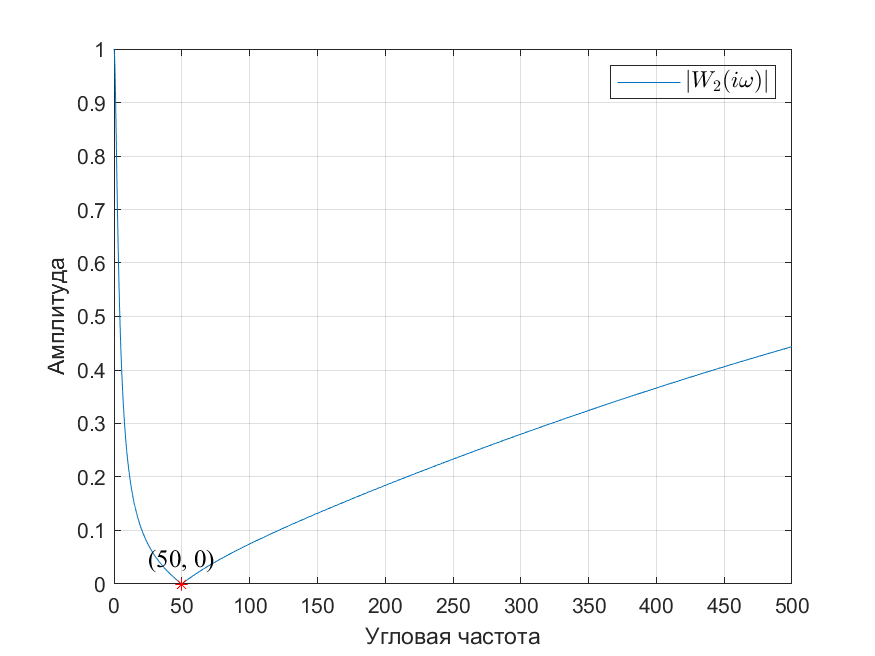
\includegraphics[width=\linewidth]{ex1_2/a1=0_a2=2500_b1=1000_b2=2500_d=50/h1.png}
        \caption{$a_1=0, a_2=2500, b_1=1000, b_2=2500$}
    \end{minipage}
\end{figure}

Видим, что чем больше $b_1$, тем больше частот около $\omega_0 = \sqrt{a_2} = 0.5$ попадает под влияние фильтра.

\subsubsection{Изучение влияния $b_1$}

Исследуем влияние параметра $b_1$ при фиксированном $d$ на эффективность фильтрации, приняв $c = 1$, $d = 5, a_1 = 0, a_2 = b_2 = 25$. При таких значениях параметра $d = \omega_0$, что обеспечит наилучшее избавление от гармонических помех. Рассмотрим графики для $b_1$ из набора $[10.5, 25, 50, 100]$, начнём с графиков АЧХ при таких параметрах:

\begin{figure}[H]
    \begin{minipage}{0.5\textwidth}
        \centering
        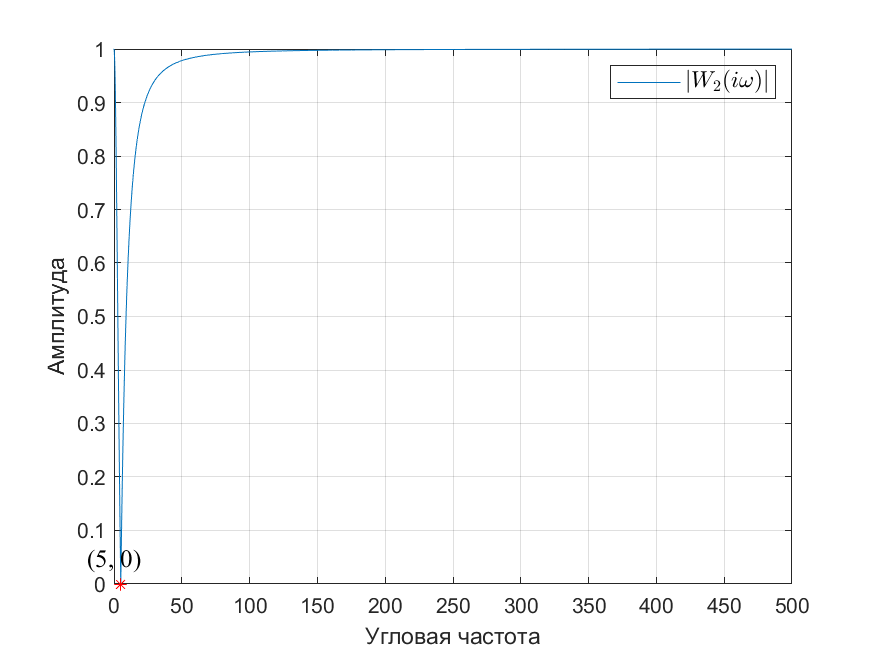
\includegraphics[width=\linewidth]{ex1_2/a1=0_a2=25_b1=10.5_b2=25_d=5/h1.png}
        \caption{АЧХ при $b_1=10.5$}
    \end{minipage}
    \begin{minipage}{0.5\textwidth}
        \centering
        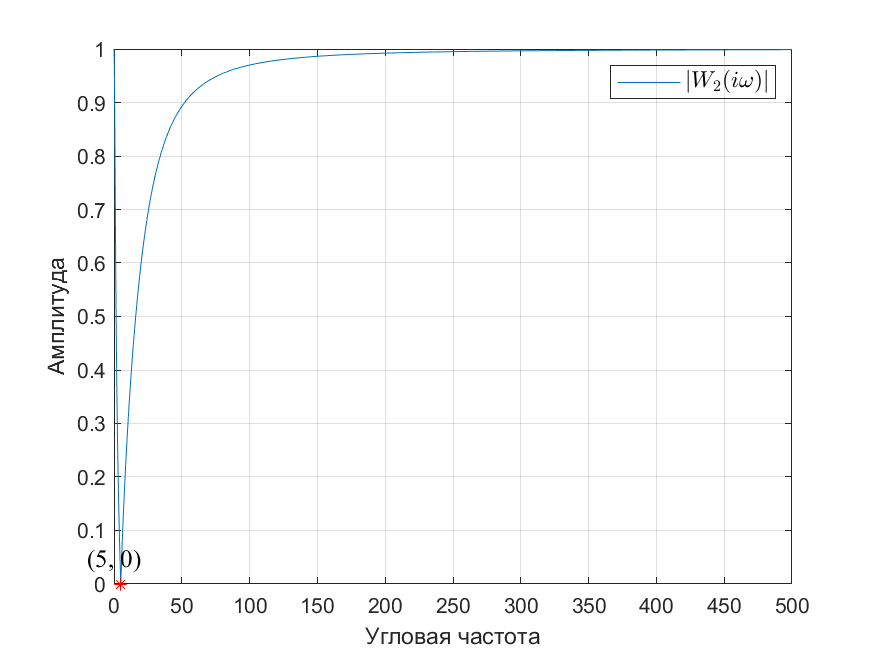
\includegraphics[width=\linewidth]{ex1_2/a1=0_a2=25_b1=25_b2=25_d=5/h1.png}
        \caption{АЧХ при $b_1=25$}
    \end{minipage}
\end{figure}

\begin{figure}[H]
    \begin{minipage}{0.5\textwidth}
        \centering
        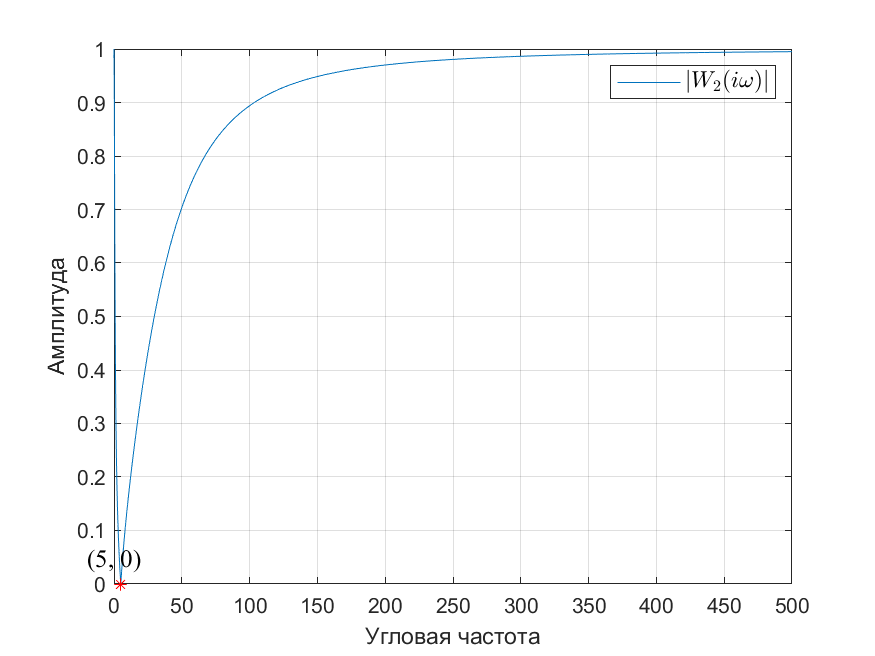
\includegraphics[width=\linewidth]{ex1_2/a1=0_a2=25_b1=50_b2=25_d=5/h1.png}
        \caption{АЧХ при $b_1=50$}
    \end{minipage}
    \begin{minipage}{0.5\textwidth}
        \centering
        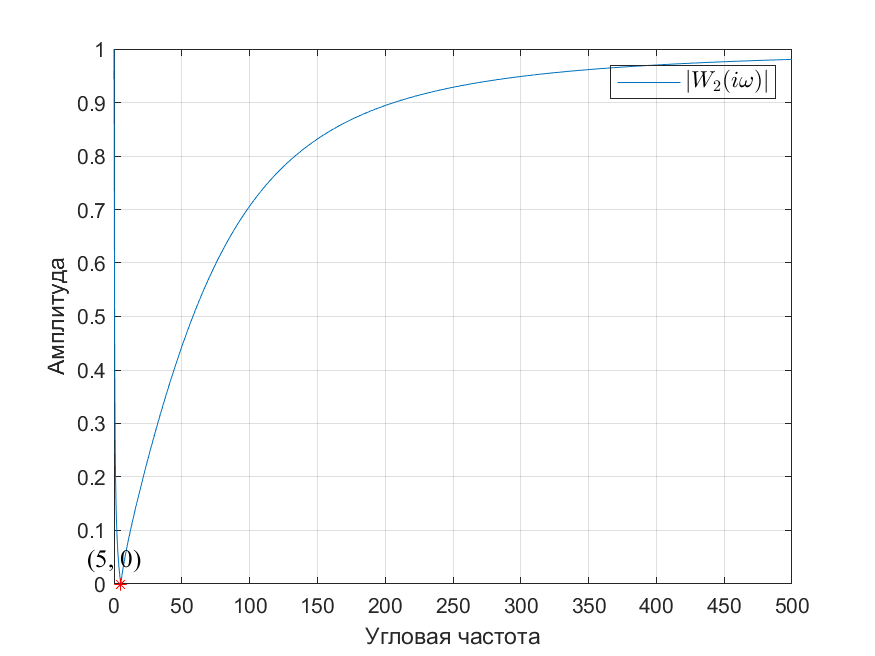
\includegraphics[width=\linewidth]{ex1_2/a1=0_a2=25_b1=100_b2=25_d=5/h1.png}
        \caption{АЧХ при $b_1=100$}
    \end{minipage}
\end{figure}

Изменение параметра $b_1$ оказывает на график АЧХ то же влияние, которое было выявлено до этого пункта -- чем больше $b_1$, тем больше частот около $\omega_0$ попадает под влияние фильтра. Убедимся в этом, посмотрев на сравнительные графики исходного, зашумлённого и фильтрованного сигналов:

\begin{figure}[H]
    \begin{minipage}{0.5\textwidth}
        \centering
        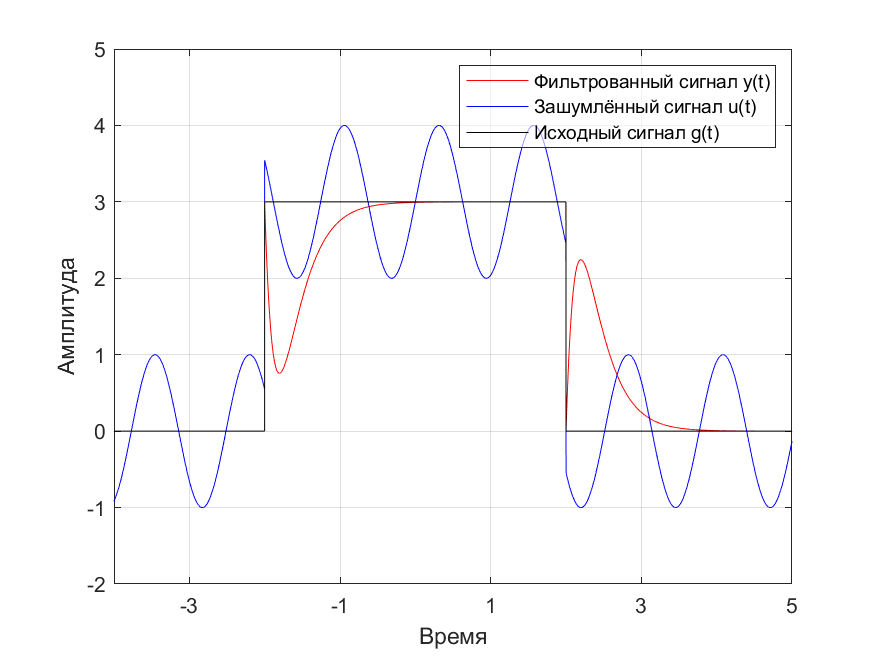
\includegraphics[width=\linewidth]{ex1_2/a1=0_a2=25_b1=10.5_b2=25_d=5/h2.png}
        \caption{$b_1=10.5$}
    \end{minipage}
    \begin{minipage}{0.5\textwidth}
        \centering
        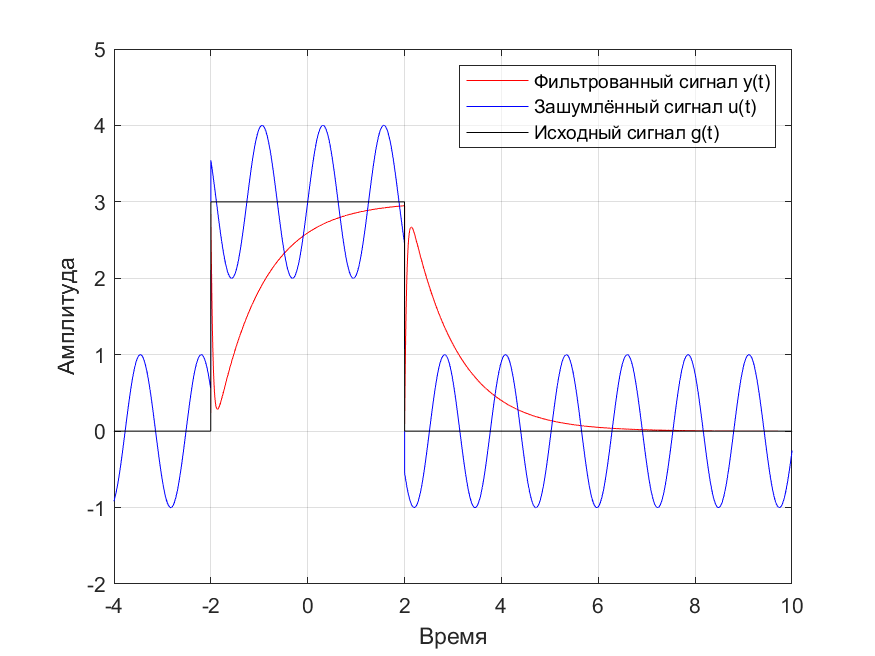
\includegraphics[width=\linewidth]{ex1_2/a1=0_a2=25_b1=25_b2=25_d=5/h2.png}
        \caption{$b_1=25$}
    \end{minipage}
\end{figure}

\begin{figure}[H]
    \begin{minipage}{0.5\textwidth}
        \centering
        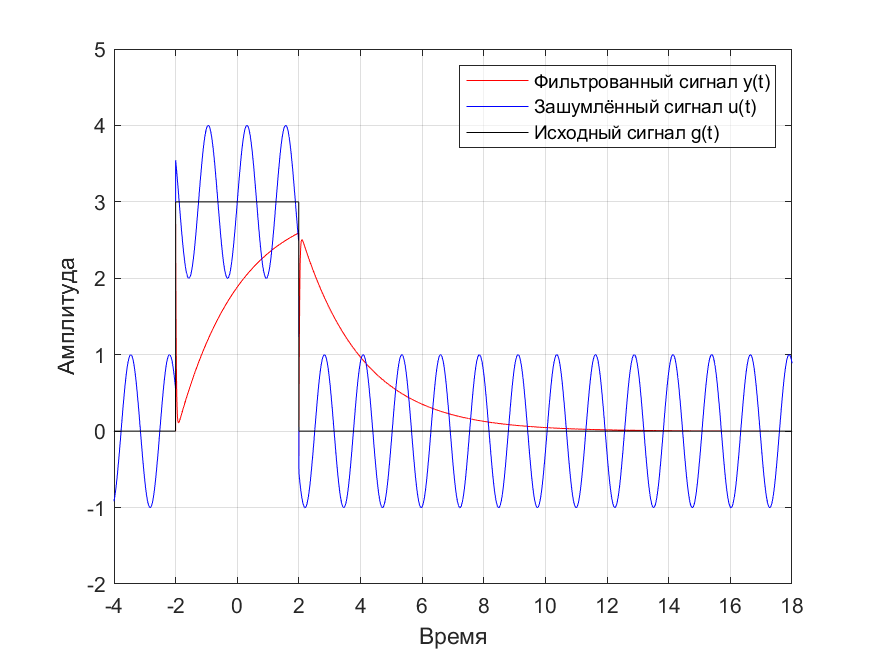
\includegraphics[width=\linewidth]{ex1_2/a1=0_a2=25_b1=50_b2=25_d=5/h2.png}
        \caption{$b_1=50$}
    \end{minipage}
    \begin{minipage}{0.5\textwidth}
        \centering
        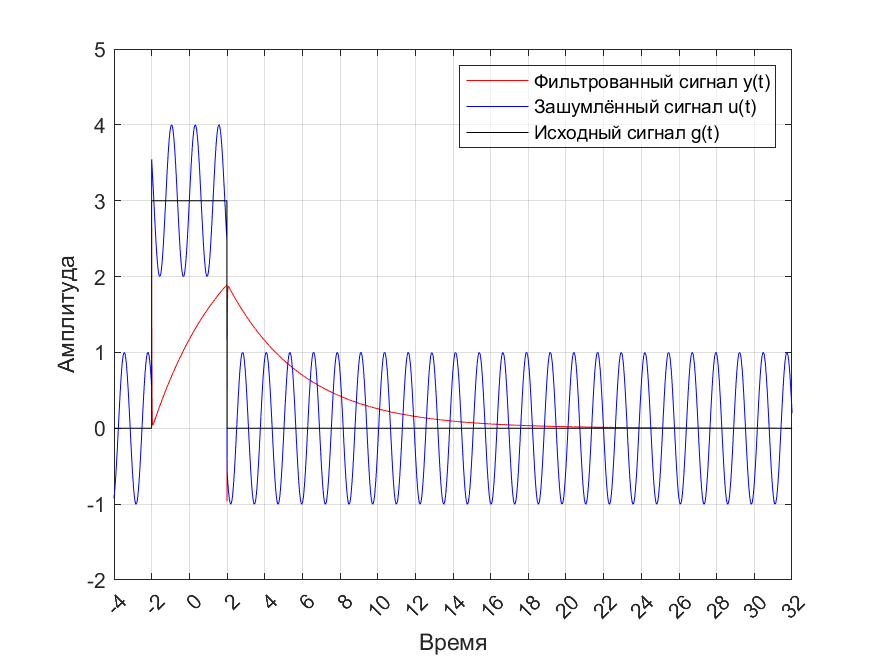
\includegraphics[width=\linewidth]{ex1_2/a1=0_a2=25_b1=100_b2=25_d=5/h2.png}
        \caption{$b_1=100$}
    \end{minipage}
\end{figure}

Замечаем, что с увеличением $b_1$ фильтр реагирует на изменения сигнала всё медленнее, и отсюда становится понятно, что большие значения этого параметра негативно сказываются на эффективности фильтрации, при этом при малых параметрах $(b_1 \leq 2\sqrt{b_2})$ фильтр перестанет быть устойчивым.

Посмотрим на графики модулей Фурье-образов этих сигналов:

\begin{figure}[H]
    \begin{minipage}{0.5\textwidth}
        \centering
        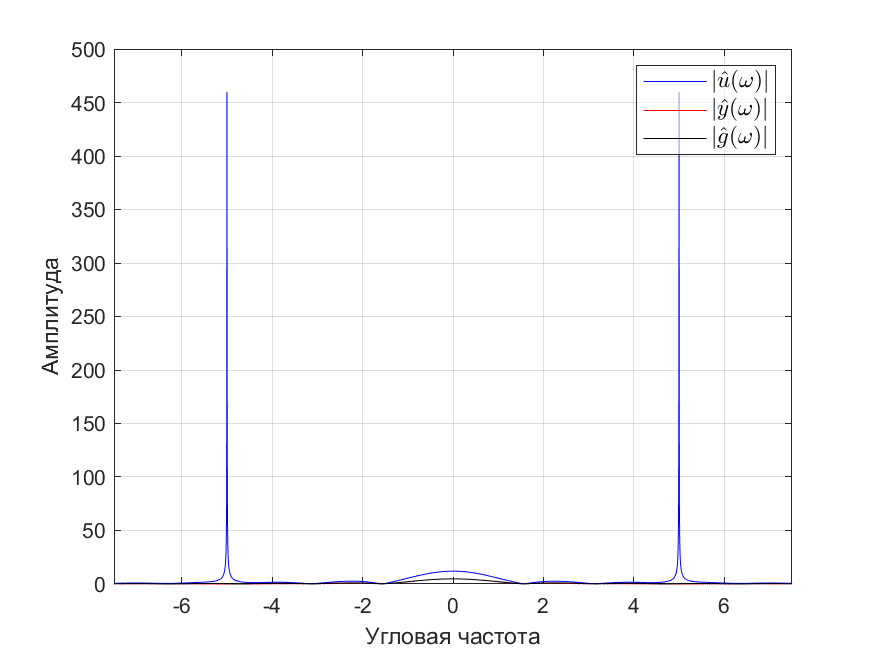
\includegraphics[width=\linewidth]{ex1_2/a1=0_a2=25_b1=10.5_b2=25_d=5/h4.png}
        \caption{$b_1=10.5$}
    \end{minipage}
    \begin{minipage}{0.5\textwidth}
        \centering
        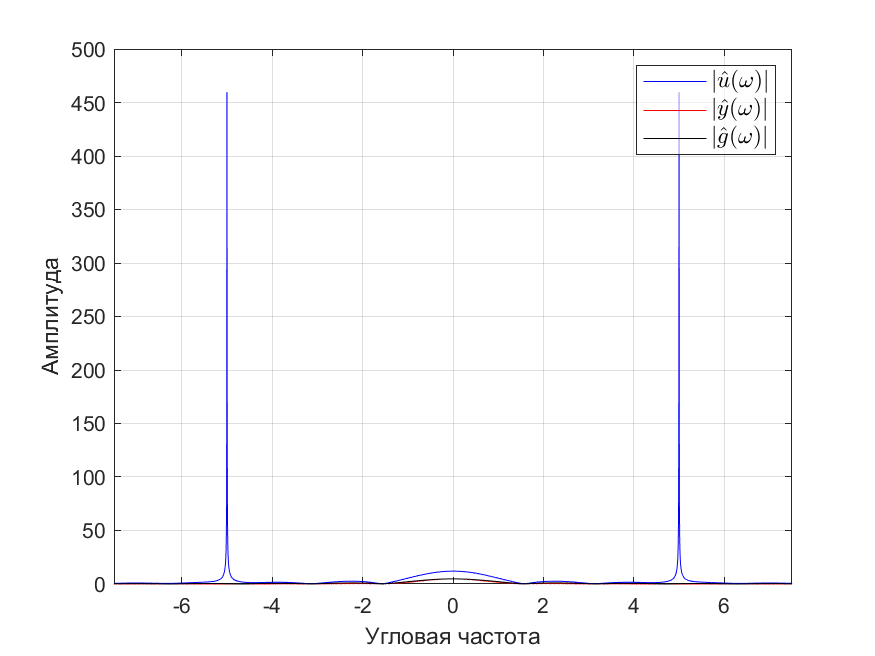
\includegraphics[width=\linewidth]{ex1_2/a1=0_a2=25_b1=25_b2=25_d=5/h4.png}
        \caption{$b_1=25$}
    \end{minipage}
\end{figure}

\begin{figure}[H]
    \begin{minipage}{0.5\textwidth}
        \centering
        \includegraphics[width=\linewidth]{ex1_2/a1=0_a2=25_b1=50_b2=25_d=5/h4.png}
        \caption{$b_1=50$}
    \end{minipage}
    \begin{minipage}{0.5\textwidth}
        \centering
        \includegraphics[width=\linewidth]{ex1_2/a1=0_a2=25_b1=100_b2=25_d=5/h4.png}
        \caption{$b_1=100$}
    \end{minipage}
\end{figure}

На каждом из рисунков видно, что график Фурье-образа зашумлённого сигнала имеет пик при $\omega = 5$, и этот пик убирается при помощи рассматриваемого фильтра. Убедимся в этом, изменив масштаб графиков:

\begin{figure}[H]
    \begin{minipage}{0.5\textwidth}
        \centering
        \includegraphics[width=\linewidth]{ex1_2/приближение/a1=0_a2=25_b1=10.5_b2=25_d=5/h4.png}
        \label{fig:d_5_b1_10.5}
        \caption{$b_1=10.5$}
    \end{minipage}
    \begin{minipage}{0.5\textwidth}
        \centering
        \includegraphics[width=\linewidth]{ex1_2/приближение/a1=0_a2=25_b1=25_b2=25_d=5/h4.png}
        \caption{$b_1=25$}
    \end{minipage}
\end{figure}

\begin{figure}[H]
    \begin{minipage}{0.5\textwidth}
        \centering
        \includegraphics[width=\linewidth]{ex1_2/приближение/a1=0_a2=25_b1=50_b2=25_d=5/h4.png}
        \caption{$b_1=50$}
    \end{minipage}
    \begin{minipage}{0.5\textwidth}
        \centering
        \includegraphics[width=\linewidth]{ex1_2/приближение/a1=0_a2=25_b1=100_b2=25_d=5/h4.png}
        \caption{$b_1=100$}
    \end{minipage}
\end{figure}

Действительно, фильтр убирает пики на графиках модулей Фурье-образов сигналов, убирая соответствующую гармонику. Однако, вместе с гармоникой убирается и часть полезного сигнала -- амплитуда фильтрованного не совпадает с амплитудой исходного, и происходит это, опять же, из-за влияния $b_1$ -- чем он больше, тем больше амплитуды теряет сигнал в процессе фильтрации. 

Следующий набор графиков:

\begin{figure}[H]
    \begin{minipage}{0.5\textwidth}
        \centering
        \includegraphics[width=\linewidth]{ex1_2/a1=0_a2=25_b1=10.5_b2=25_d=5/h3.png}
        \caption{$b_1=10.5$}
    \end{minipage}
    \begin{minipage}{0.5\textwidth}
        \centering
        \includegraphics[width=\linewidth]{ex1_2/a1=0_a2=25_b1=25_b2=25_d=5/h3.png}
        \caption{$b_1=25$}
    \end{minipage}
\end{figure}

\begin{figure}[H]
    \begin{minipage}{0.5\textwidth}
        \centering
        \includegraphics[width=\linewidth]{ex1_2/a1=0_a2=25_b1=50_b2=25_d=5/h3.png}
        \caption{$b_1=50$}
    \end{minipage}
    \begin{minipage}{0.5\textwidth}
        \centering
        \includegraphics[width=\linewidth]{ex1_2/a1=0_a2=25_b1=100_b2=25_d=5/h3.png}
        \caption{$b_1=100$}
    \end{minipage}
\end{figure}

На приведенных графиках $y(t)$ -- фильтрованный сигнал, полученный при помощи функции функции $lsim$ из $MATLAB$, и он полностью совпадает с фильтрованным сигналом, полученным в результате обратного преобразования Фурье от произведения фильтра и Фурье-образа зашумлённой функции, что подтверждает равенство $y = \mathcal{F}^{-1}\{W_2(i \omega) \hat{u}\}$, рассмотренное на лекции.

Графики Фурье-образов фильтрованного сигнала, полученного при помощи $lsim$ из $MATLAB$, и фильтрованного сигнала, полученного по формуле $W_2(i \omega) \cdot \hat{u}(\omega)$:

\begin{figure}[H]
    \begin{minipage}{0.5\textwidth}
        \centering
        \includegraphics[width=\linewidth]{ex1_2/a1=0_a2=25_b1=10.5_b2=25_d=5/h5.png}
        \caption{$b_1=10.5$}
    \end{minipage}
    \begin{minipage}{0.5\textwidth}
        \centering
        \includegraphics[width=\linewidth]{ex1_2/a1=0_a2=25_b1=25_b2=25_d=5/h5.png}
        \caption{$b_1=25$}
    \end{minipage}
\end{figure}

\begin{figure}[H]
    \begin{minipage}{0.5\textwidth}
        \centering
        \includegraphics[width=\linewidth]{ex1_2/a1=0_a2=25_b1=50_b2=25_d=5/h5.png}
        \caption{$b_1=50$}
    \end{minipage}
    \begin{minipage}{0.5\textwidth}
        \centering
        \includegraphics[width=\linewidth]{ex1_2/a1=0_a2=25_b1=100_b2=25_d=5/h5.png}
        \caption{$b_1=100$}
    \end{minipage}
\end{figure}

Графики снова очень похожи, обе версии фильтра убирают гармоники при $\omega_0$, стремятся к нулю на бесконечности, при увеличении $b_1$ снижаются амплитуды, однако график Фурье-образа сигнала, полученного через встроенную в $MATLAB$ функцию, ``сформирован'' из мелких колебаний (\textit{я не знаю как именно это описать\ldots}). Это связано с тем, как реализована встроенная функция $lsim$ -- возможно, это следствие её оптимизации.

\subsubsection{Изучение влияния $d$}

Зафиксируем $b_1 = 10.5$ при прочих неизменных параметрах $c = 1, a_1 = 0, a_2 = b_2 = 25$ и посмотрим, как изменится эффективность фильтрации при варьировании $d$. При построении графиков будут взяты $d$ из набора $[1, 5, 10, 20]$. Начнем с графиков сигналов:

\begin{figure}[H]
    \begin{minipage}{0.5\textwidth}
        \centering
        \includegraphics[width=\linewidth]{ex1_2/a1=0_a2=25_b1=10.5_b2=25_d=1/h2.png}
        \caption{$d=1$}
    \end{minipage}
    \begin{minipage}{0.5\textwidth}
        \centering
        \includegraphics[width=\linewidth]{ex1_2/a1=0_a2=25_b1=10.5_b2=25_d=5/h2.png}
        \caption{$d=5$}
    \end{minipage}
\end{figure}

\begin{figure}[H]
    \begin{minipage}{0.5\textwidth}
        \centering
        \includegraphics[width=\linewidth]{ex1_2/a1=0_a2=25_b1=10.5_b2=25_d=10/h2.png}
        \caption{$d=10$}
    \end{minipage}
    \begin{minipage}{0.5\textwidth}
        \centering
        \includegraphics[width=\linewidth]{ex1_2/a1=0_a2=25_b1=10.5_b2=25_d=20/h2.png}
        \caption{$d=20$}
    \end{minipage}
\end{figure}

Видим, что чем больше значение параметра $d$, тем больше частота гармонического шума. Графики Фурье-образов этих сигналов:

\begin{figure}[H]
    \begin{minipage}{0.5\textwidth}
        \centering
        \includegraphics[width=\linewidth]{ex1_2/a1=0_a2=25_b1=10.5_b2=25_d=1/h4.png}
        \caption{$d=1$}
    \end{minipage}
    \begin{minipage}{0.5\textwidth}
        \centering
        \includegraphics[width=\linewidth]{ex1_2/a1=0_a2=25_b1=10.5_b2=25_d=5/h4.png}
        \caption{$d=5$}
    \end{minipage}
\end{figure}

\begin{figure}[H]
    \begin{minipage}{0.5\textwidth}
        \centering
        \includegraphics[width=\linewidth]{ex1_2/a1=0_a2=25_b1=10.5_b2=25_d=10/h4.png}
        \caption{$d=10$}
    \end{minipage}
    \begin{minipage}{0.5\textwidth}
        \centering
        \includegraphics[width=\linewidth]{ex1_2/a1=0_a2=25_b1=10.5_b2=25_d=20/h4.png}
        \caption{$d=20$}
    \end{minipage}
\end{figure}

Из приведённых рисунков видно, что пики на графиках модулей Фурье-образов появляются именно при $\omega = d$. При таком значении параметров $a_2 = b_2$ гармонические колебания будут убраны только при $d = \sqrt{a_2} = 5$, то есть на втором графике, который уже был рассмотрен в более наглядном масштабе в пункте \ref{fig:d_5_b1_10.5}, для остальных графиков пик не будет отфильтрован.

Снова сравним реализацию действия фильтра на сигнал при помощи $lsim$ и при помощи формулы, рассмотренной на лекции: 

\begin{figure}[H]
    \begin{minipage}{0.5\textwidth}
        \centering
        \includegraphics[width=\linewidth]{ex1_2/a1=0_a2=25_b1=10.5_b2=25_d=1/h3.png}
        \caption{$d=1$}
    \end{minipage}
    \begin{minipage}{0.5\textwidth}
        \centering
        \includegraphics[width=\linewidth]{ex1_2/a1=0_a2=25_b1=10.5_b2=25_d=5/h3.png}
        \caption{$d=5$}
    \end{minipage}
\end{figure}

\begin{figure}[H]
    \begin{minipage}{0.5\textwidth}
        \centering
        \includegraphics[width=\linewidth]{ex1_2/a1=0_a2=25_b1=10.5_b2=25_d=10/h3.png}
        \caption{$d=10$}
    \end{minipage}
    \begin{minipage}{0.5\textwidth}
        \centering
        \includegraphics[width=\linewidth]{ex1_2/a1=0_a2=25_b1=10.5_b2=25_d=20/h3.png}
        \caption{$d=20$}
    \end{minipage}
\end{figure}

Снова графики сходятся, что демонстрирует выполнение равенства $y = \mathcal{F}^{-1}\{W_2(i \omega) \hat{u}\}$. Посмотрим на графики Фурье-образов фильтрованных сигналов, полученных разными способами:

\begin{figure}[H]
    \begin{minipage}{0.5\textwidth}
        \centering
        \includegraphics[width=\linewidth]{ex1_2/a1=0_a2=25_b1=10.5_b2=25_d=1/h5.png}
        \caption{$d=1$}
    \end{minipage}
    \begin{minipage}{0.5\textwidth}
        \centering
        \includegraphics[width=\linewidth]{ex1_2/a1=0_a2=25_b1=10.5_b2=25_d=5/h5.png}
        \caption{$d=5$}
    \end{minipage}
\end{figure}

\begin{figure}[H]
    \begin{minipage}{0.5\textwidth}
        \centering
        \includegraphics[width=\linewidth]{ex1_2/a1=0_a2=25_b1=10.5_b2=25_d=10/h5.png}
        \caption{$d=10$}
    \end{minipage}
    \begin{minipage}{0.5\textwidth}
        \centering
        \includegraphics[width=\linewidth]{ex1_2/a1=0_a2=25_b1=10.5_b2=25_d=20/h5.png}
        \caption{$d=20$}
    \end{minipage}
\end{figure}

Видим, что графики совпадают.

\subsubsection{Изучение влияния $c$}

Зафиксируем $d$, примем его равным $d = 5$ при прочих неизменных параметрах: $a_1 = 0, b_1 = 10.5, a_2 = b_2 = 25$, исследуем влияние коэффициента $c$ на эффективность фильтрации. Рассмотрим графики исходного, зашумлённого, фильтрованного сигналов при $c \in [1, 2, 5, 10]$:

\begin{figure}[H]
    \begin{minipage}{0.5\textwidth}
        \centering
        \includegraphics[width=\linewidth]{ex1_2/a1=0_a2=25_b1=10.5_b2=25_d=5_c=1/h2.png}
        \caption{$c=1$}
    \end{minipage}
    \begin{minipage}{0.5\textwidth}
        \centering
        \includegraphics[width=\linewidth]{ex1_2/a1=0_a2=25_b1=10.5_b2=25_d=5_c=2/h2.png}
        \caption{$c=2$}
    \end{minipage}
\end{figure}

\begin{figure}[H]
    \begin{minipage}{0.5\textwidth}
        \centering
        \includegraphics[width=\linewidth]{ex1_2/a1=0_a2=25_b1=10.5_b2=25_d=5_c=5/h2.png}
        \caption{$c=5$}
    \end{minipage}
    \begin{minipage}{0.5\textwidth}
        \centering
        \includegraphics[width=\linewidth]{ex1_2/a1=0_a2=25_b1=10.5_b2=25_d=5_c=10/h2.png}
        \caption{$c=10$}
    \end{minipage}
\end{figure}

Видим, что хоть значение параметра $c$ увеличивает амплитуду шумов, оно не влияет на эффективность фильтрации при $d = \omega_0 = 5$, так как в любом случае гармоника, на которой находятся гармонические шумы, зануляется. Рассмотрим случаи с $d = 4$:

\begin{figure}[H]
    \begin{minipage}{0.5\textwidth}
        \centering
        \includegraphics[width=\linewidth]{ex1_2/a1=0_a2=25_b1=10.5_b2=25_d=4_c=1/h2.png}
        \caption{$c=1$}
    \end{minipage}
    \begin{minipage}{0.5\textwidth}
        \centering
        \includegraphics[width=\linewidth]{ex1_2/a1=0_a2=25_b1=10.5_b2=25_d=4_c=2/h2.png}
        \caption{$c=2$}
    \end{minipage}
\end{figure}

\begin{figure}[H]
    \begin{minipage}{0.5\textwidth}
        \centering
        \includegraphics[width=\linewidth]{ex1_2/a1=0_a2=25_b1=10.5_b2=25_d=4_c=5/h2.png}
        \caption{$c=5$}
    \end{minipage}
    \begin{minipage}{0.5\textwidth}
        \centering
        \includegraphics[width=\linewidth]{ex1_2/a1=0_a2=25_b1=10.5_b2=25_d=4_c=10/h2.png}
        \caption{$c=10$}
    \end{minipage}
\end{figure}

Видно, что увеличение значения $c$ приводит к увеличению амплитуды колебаний зашумлённого сигнала, а то в свою очередь -- у увеличению амплитуды колебаний фильтрованного сигнала. Рассмотрим графики модулей Фурье-образов этих сигналов:

\begin{figure}[H]
    \begin{minipage}{0.5\textwidth}
        \centering
        \includegraphics[width=\linewidth]{ex1_2/a1=0_a2=25_b1=10.5_b2=25_d=4_c=1/h4.png}
        \caption{$c=1$}
    \end{minipage}
    \begin{minipage}{0.5\textwidth}
        \centering
        \includegraphics[width=\linewidth]{ex1_2/a1=0_a2=25_b1=10.5_b2=25_d=4_c=2/h4.png}
        \caption{$c=2$}
    \end{minipage}
\end{figure}

\begin{figure}[H]
    \begin{minipage}{0.5\textwidth}
        \centering
        \includegraphics[width=\linewidth]{ex1_2/a1=0_a2=25_b1=10.5_b2=25_d=4_c=5/h4.png}
        \caption{$c=5$}
    \end{minipage}
    \begin{minipage}{0.5\textwidth}
        \centering
        \includegraphics[width=\linewidth]{ex1_2/a1=0_a2=25_b1=10.5_b2=25_d=4_c=10/h4.png}
        \caption{$c=10$}
    \end{minipage}
\end{figure}

Как можно заметить, модули Фурье-образов также увеличиваются в амплитуде при $\omega = d = 4$, соразмерно с увеличением $c$. Немного приблизим график для большей наглядности:

\begin{figure}[H]
    \begin{minipage}{0.5\textwidth}
        \centering
        \includegraphics[width=\linewidth]{ex1_2/приближение/a1=0_a2=25_b1=10.5_b2=25_d=4_c=1/h4.png}
        \caption{$c=1$}
    \end{minipage}
    \begin{minipage}{0.5\textwidth}
        \centering
        \includegraphics[width=\linewidth]{ex1_2/приближение/a1=0_a2=25_b1=10.5_b2=25_d=4_c=2/h4.png}
        \caption{$c=2$}
    \end{minipage}
\end{figure}

\begin{figure}[H]
    \begin{minipage}{0.5\textwidth}
        \centering
        \includegraphics[width=\linewidth]{ex1_2/приближение/a1=0_a2=25_b1=10.5_b2=25_d=4_c=5/h4.png}
        \caption{$c=5$}
    \end{minipage}
    \begin{minipage}{0.5\textwidth}
        \centering
        \includegraphics[width=\linewidth]{ex1_2/приближение/a1=0_a2=25_b1=10.5_b2=25_d=4_c=10/h4.png}
        \caption{$c=10$}
    \end{minipage}
\end{figure}

Видим, что гармоники $\omega \ne d$ остаются неизменными, если не брать во внимание увеличение ``ширины'' линии модуля образа фильтрованного сигнала (\textit{на самом деле ширина увеличивается за счёт увеличения амплитуд мелких колебаний, появляющихся при использовании $lsim$}).

Сравним графики модулей образов фильтрованных сигналов, полученных встроенной функцией и по формуле умножения фильтра на Фурье-образ зашумленного сигнала:

\begin{figure}[H]
    \begin{minipage}{0.5\textwidth}
        \centering
        \includegraphics[width=\linewidth]{ex1_2/приближение/a1=0_a2=25_b1=10.5_b2=25_d=4_c=1/h5.png}
        \caption{$c=1$}
    \end{minipage}
    \begin{minipage}{0.5\textwidth}
        \centering
        \includegraphics[width=\linewidth]{ex1_2/приближение/a1=0_a2=25_b1=10.5_b2=25_d=4_c=2/h5.png}
        \caption{$c=2$}
    \end{minipage}
\end{figure}

\begin{figure}[H]
    \begin{minipage}{0.5\textwidth}
        \centering
        \includegraphics[width=\linewidth]{ex1_2/приближение/a1=0_a2=25_b1=10.5_b2=25_d=4_c=5/h5.png}
        \caption{$c=5$}
    \end{minipage}
    \begin{minipage}{0.5\textwidth}
        \centering
        \includegraphics[width=\linewidth]{ex1_2/приближение/a1=0_a2=25_b1=10.5_b2=25_d=4_c=10/h5.png}
        \caption{$c=10$}
    \end{minipage}
\end{figure}

Видно, что при больших $c$ заметны расхождения в графиках этих функций, посмотрим, повлияют ли эти расхождения на конечный результат:

\begin{figure}[H]
    \begin{minipage}{0.5\textwidth}
        \centering
        \includegraphics[width=\linewidth]{ex1_2/a1=0_a2=25_b1=10.5_b2=25_d=4_c=1/h3.png}
        \caption{$c=1$}
    \end{minipage}
    \begin{minipage}{0.5\textwidth}
        \centering
        \includegraphics[width=\linewidth]{ex1_2/a1=0_a2=25_b1=10.5_b2=25_d=4_c=2/h3.png}
        \caption{$c=2$}
    \end{minipage}
\end{figure}

\begin{figure}[H]
    \begin{minipage}{0.5\textwidth}
        \centering
        \includegraphics[width=\linewidth]{ex1_2/a1=0_a2=25_b1=10.5_b2=25_d=4_c=5/h3.png}
        \caption{$c=5$}
    \end{minipage}
    \begin{minipage}{0.5\textwidth}
        \centering
        \includegraphics[width=\linewidth]{ex1_2/a1=0_a2=25_b1=10.5_b2=25_d=4_c=10/h3.png}
        \caption{$c=10$}
    \end{minipage}
\end{figure}

Отличий в результирующем сигнале на графиках не заметно, несмотря на незначительные отличия в Фурье-образах. Чем больше значение параметра $c$, тем больше колебания, и тем ниже эффективность фильтрации выбранным фильтром.

\subsubsection{Вывод}\

Гармонические шумы могут быть отфильтрованы рассмотренным фильтром с большой эффективностью, если $d = \omega_0$, где $\omega_0 = \sqrt{a_2} = \sqrt{b_2}$ -- частота, амплитуду на которой фильтр делает равной нулю. Однако чем больше $b_1$, тем большее кол-во частот около $\omega_0$ захватывает фильтр, влияя в том числе и на полезный сигнал, самым эффективным $b_1$ оказалось значение немного большее $2\sqrt{b_2}$ -- при таком значении гармонический шум пропадает, и остальные гармоники фильтр почти не захватывает.

\subsection{Выводы}\

Фильтр первого порядка позволяет избавиться от случайного шума, режекторный полосовой фильтр -- от гармонического, исследовано влияние параметров на эффективность такой фильтрации.

\section{Сглаживание биржевых данных}\

Для выполнения этого задания я скачал данные о стоимости акций Сбербанка за прошедший год, загрузил их в $MATLAB$, вычел из всех значений получившегося сигнала первое, чтобы первое значение стало равным нулю, и данные корректно обработались функцией $lsim$, после применения линейного фильтра первого порядка прибавил к каждому элементу фильтрованного сигнала первое значение исходного (которое сначала вычел), и получил корректные данные:

\begin{figure}[H]
    \centering
    \includegraphics[width=\linewidth]{ex2/1.png}
    \caption{Сглаживание за 1 день, $T = 1$}
\end{figure}

\begin{figure}[H]
    \centering
    \includegraphics[width=\linewidth]{ex2/7.png}
    \caption{Сглаживание за неделю, $T = 7$}
\end{figure}

\begin{figure}[H]
    \centering
    \includegraphics[width=\linewidth]{ex2/30.png}
    \caption{Сглаживание за месяц, $T = 30$}
\end{figure}

\begin{figure}[H]
    \centering
    \includegraphics[width=\linewidth]{ex2/90.png}
    \caption{Сглаживание за 3 месяца, $T = 90$}
\end{figure}

\begin{figure}[H]
    \centering
    \includegraphics[width=\linewidth]{ex2/365.png}
    \caption{Сглаживание за год, $T = 365$}
\end{figure}

\subsection{Выводы}\

В результате выполнения задания я усвоил, что фильтр первого порядка можно использовать не только для устранения шумов, но и для аппроксимации поступающего сигнала (что в некотором смысле одно и то же).

\section{Вывод по работе}\

В процессе выполнения работы я познакомился с динамической фильтрацией, с двумя фильтрами, реализующими такую фильтрацию, проанализировал их, понял, как при их помощи можно наиболее эффективно избавиться от гармонического и белого шума, также при сравнении фильтрованного через $lsim$ сигнала с сигналом, полученным после обратного преобразования Фурье произведения частотной передаточной функции фильтра и образа зашумленного сигнала убедился в том, что теорема о свёртке работает, и это избавляет от необходимости находить решение дифференциального уравнения, соответствующего передаточной функции, при обработке сигналов.

\end{document}
